\documentclass[pdftex]{pucthesis}

% Floats
\usepackage{graphicx}
\usepackage{float}
\usepackage{color}
\usepackage{pgfgantt}
\usepackage{chngcntr}
\counterwithin{figure}{chapter}
\counterwithin{table}{chapter}

% Matemáticas
\usepackage{amsmath}
\usepackage{amsfonts}
\usepackage{amssymb}

% Times
\usepackage{times}

% Tablas
\usepackage{booktabs}
\usepackage{multirow}
\usepackage{tabularx}
\usepackage{array}
\usepackage[table]{xcolor}
\newcolumntype{Y}{>{\raggedright\arraybackslash}X}
\newcolumntype{R}{>{\raggedleft\arraybackslash}X}

% Algoritmos y diagramas
\usepackage{tikz}
\usetikzlibrary{positioning,arrows.meta,shapes.geometric,fit,calc}
\usepackage[ruled,linesnumbered,vlined]{algorithm2e}
\SetAlgorithmName{Algoritmo}{Algoritmo}{Lista de algoritmos}
\SetKwInput{KwIn}{Entrada}
\SetKwInput{KwOut}{Salida}

\usepackage{etoolbox}
\apptocmd{\sloppy}{\hbadness 10000\relax}{}{}

% Citas y referencias
\usepackage[hidelinks,pdfusetitle,pdfdisplaydoctitle]{hyperref}
\usepackage[notocbib]{apacite}
\usepackage{doi}
\renewcommand{\doitext}{}

\usepackage[spanish,es-nodecimaldot,es-tabla]{babel}
\addto\captionsspanish{\renewcommand{\chaptername}{}}

\usepackage{caption}
\captionsetup{font=small,labelfont=bf}
\setlength{\abovecaptionskip}{4pt}
\setlength{\belowcaptionskip}{2pt}
\setlength{\textfloatsep}{10pt plus 2pt minus 2pt}
\setlength{\floatsep}{8pt plus 2pt minus 2pt}
\setlength{\intextsep}{8pt plus 2pt minus 2pt}
\raggedbottom
\clubpenalty=150
\widowpenalty=150

\newcommand{\parrafo}[1]{\par\smallskip\noindent\textbf{#1}\ }
\makeatletter\newcommand{\tabinput}[1]{\@@input #1 }\makeatother
\begin{document}

\title[Diseño y optimización de la red semanal de transporte sanitario\\ GRUPO 12]
   {\bf Diseño y optimización de la red semanal de transporte sanitario\\ GRUPO 12}
\author[Integrantes:]{Integrantes:\\
\textnormal{\small{
Josefina Pérez Prochelle\\
Nicolás Prohens Martínez\\
Antonia Rivera Mujica\\
Pedro Sanzana Santander\\
Luis Uribe Baeza\\
Isabel Wilhelmy Vergara}}}
\address{Escuela de Ingenier\'ia\\ Pontificia Universidad Cat\'olica de Chile}
\advisor{\textbf{Profesor Guía:} Francisco Tamarín Salinas}
\ogrsmember{\textbf{Ayudante Tutor:} Martín Tuset Cuevas}
\date{2026}
\copyrightname{Grupo 12}
\copyrightyear{2026}

\NoChapterPageNumber
\pagenumbering{roman}
\maketitle

\chapter*{DECLARACIÓN DE USO DE INTELIGENCIA ARTIFICIAL}
\noindent Grupo: 12

\vspace{0.4cm}
\noindent ¿Hicieron uso de herramientas de IA en su trabajo para este informe y/o presentación? \quad SÍ \underline{\ X\ } \quad NO \underline{\ \ \ \ }

\vspace{0.4cm}
\noindent ¿Cuáles de las siguientes alternativas mejor describe el uso que hicieron de IA (puede ser más de una)?

\vspace{0.2cm}
\noindent
\begin{tabular}{@{}p{0.04\textwidth} p{0.92\textwidth}@{}}
\checkmark & Apoyo a la redacción, ortografía, estructura gramatical, etc., de los documentos. \\
\checkmark & Apoyo al análisis de datos e información asociada al problema. \\
\checkmark & Búsqueda y/o filtro de referencias, contenidos web, literatura, etc., relevante al proyecto. \\
\checkmark & Apoyo para el desarrollo de modelos asociados al proyecto. \\
\checkmark & Apoyo en el desarrollo de código computacional necesario para el proyecto. \\
\checkmark & Apoyo en el análisis de resultados (por ejemplo, de distintas corridas computacionales). \\
\checkmark & Apoyo para construir figuras, diagramas, etc. \\
 & Apoyo para obtener conclusiones a partir de los análisis de resultados. \\
 & Otro, especificar: \rule{8cm}{0.4pt}
\end{tabular}

\vspace{0.3cm}
\noindent Chats de IA utilizados: Claude (Anthropic).

\vspace{0.3cm}
\noindent Reflexión. La IA fue un apoyo útil para comunicar con mayor precisión las ideas dentro del límite de páginas y para repasar la teoría antes de elegir las metodologías. En esta versión fue especialmente útil para auditar el código: ayudó a encontrar inconsistencias entre lo implementado y lo descrito, a perfilar el tiempo de cómputo y a programar las figuras. Todas las decisiones de modelación, la interpretación de los resultados y las conclusiones fueron revisadas y validadas por el grupo, y cada cifra del informe proviene de una corrida reproducible del código entregado.

\vspace{0.4cm}
\noindent Esta declaración debe ser firmada por todos los integrantes del grupo:

\vspace{0.2cm}
\noindent
\begin{tabular}{@{}p{0.31\textwidth}p{0.31\textwidth}p{0.31\textwidth}@{}}

\includegraphics[height=1.4cm]{firmas/josefina.jpeg} & 
\includegraphics[height=1.4cm]{firmas/nicolas.png} & 
\includegraphics[height=1.4cm]{firmas/antonia.png} \\
Josefina Pérez Prochelle & Nicolás Prohens Martínez & Antonia Rivera Mujica \\[0.5cm]

\includegraphics[height=1.4cm]{firmas/pedro.png} & 
\includegraphics[height=1.4cm]{firmas/luis.jpeg} & 
\includegraphics[height=1.4cm]{firmas/isa.jpeg} \\
Pedro Sanzana Santander & Luis Uribe Baeza & Isabel Wilhelmy Vergara
\end{tabular}

\cleardoublepage

\pdfbookmark{\contentsname}{toc}
\tableofcontents
\cleardoublepage

\pagenumbering{arabic}

\chapter[ABSTRACT]{Abstract}
A healthcare transport network in the Santiago Metropolitan Region must decide every week how many vehicles to hire, where to station them and which transfer hubs to open, and every day how to serve between 455 and 731 weekly requests for clinical samples, refrigerated drugs, supplies and equipment. This report proposes a matheuristic that coordinates both levels. GRASP and VND heuristics generate feasible daily routes, a set-partitioning model solved with Gurobi selects the fleet, bases, hubs and service mode of each request, and a dual-based column generation adds routes that can lower the cost. Compared with a rule-based baseline, the matheuristic is cheaper in all 80 available weeks, saving 9.9\,\% on the large instances (3.9 million CLP per week) and 15.7\,\% on the small ones, mostly by routing 16\,\% fewer kilometres with almost the same fleet. The savings are statistically significant, stable across random seeds, and hold in every sensitivity scenario. Refrigerated vans are the binding resource, and splitting requests across vehicles is essential, while transfer hubs add little value. No base is indispensable and an additional base does not pay off, whereas two extra vans in high-demand weeks reduce cost and outsourcing. A staged implementation with a shadow run and a zone pilot is proposed.

\vspace{0.5em}
\noindent\textbf{Keywords:} vehicle routing, fleet sizing, matheuristic, column generation, healthcare logistics.


\chapter[RESUMEN EJECUTIVO]{Resumen ejecutivo}\label{cap:resumen}
Una red de transporte sanitario de la Región Metropolitana debe decidir cada semana cuántos vehículos contratar, en qué bases ubicarlos y qué hubs habilitar, y cada día cómo atender entre 455 y 731 solicitudes semanales de muestras clínicas, fármacos refrigerados, insumos y equipos. Hoy esas decisiones se toman por separado y con reglas simples. Este informe propone una herramienta que las coordina.

\parrafo{Método.} La herramienta es una matheurística. Heurísticas GRASP y VND generan rutas diarias factibles; un modelo de particionamiento de conjuntos resuelto con Gurobi elige entre ellas la flota, las bases, los hubs y la forma de atender cada solicitud; y una generación de columnas con los precios duales del modelo agrega rutas que pueden bajar el costo. Se compara contra un caso base que representa la planificación por reglas: dimensiona la flota según la demanda e inserta cada solicitud en la ruta más barata. Un validador independiente revisa que cada solución cumpla todas las restricciones.

\parrafo{Resultados.} La matheurística es más barata que el caso base en las 80 semanas disponibles: un 9,9\,\% en las 40 semanas BIG (\$3,9 millones por semana) y un 15,7\,\% en las 40 SMALL. La diferencia es estadísticamente significativa y casi no depende de la semilla. El ahorro viene de rutear mejor: con casi la misma flota recorre un 16\,\% menos de kilómetros y externaliza un 28\,\% menos. Una semana BIG se resuelve en unos 25 minutos en un computador personal.

\parrafo{Diagnóstico.} El recurso escaso es el furgón frío: en 26 de las 40 semanas BIG se usan los 18 disponibles, y las solicitudes difíciles son insumos y equipos grandes con ventanas de una hora. La división de solicitudes entre vehículos es esencial (sin ella el costo sube un tercio), mientras que los hubs casi no aportan con estos datos.

\parrafo{Sensibilidad e infraestructura.} En 60 corridas de sensibilidad la ventaja se mantuvo en todos los escenarios. Lo que más mueve el costo es la demanda, que lo hace crecer más que proporcionalmente, y la congestión, que lo sube hasta un 11\,\%. Exigir puntualidad total no encarece la operación. Ninguna base es imprescindible, una décima base no paga su costo y la capacidad de las bases no limita; en cambio, dos furgones adicionales en las semanas de alta demanda bajan el costo y las externalizaciones.

\parrafo{Recomendaciones.} Se recomienda (1) implementar la herramienta en tres etapas, con una marcha blanca de cuatro semanas, un piloto de ocho semanas en las bases del poniente y el despliegue completo; (2) contratar dos furgones adicionales en forma flexible para las semanas de alta demanda; (3) negociar ventanas de atención más amplias con los centros que más externalizan, porque media hora más baja el costo cerca de un 4\,\%; (4) exigir puntualidad total, que no tiene costo; y (5) evaluar con más semanas el cierre de Talagante. Las principales limitaciones son que la solución es aproximada, que los tiempos de viaje suponen flujo libre y que la demanda se supone conocida al inicio de la semana.


\chapter[INTRODUCCIÓN]{Introducción}
Los sistemas de salud dependen de una logística que el paciente rara vez ve. Para que un examen se procese, un tratamiento se administre o un pabellón funcione, alguien tiene que llevar a tiempo una muestra al laboratorio, un medicamento refrigerado a la farmacia o un equipo de vuelta a su centro de reposición. Cuando ese transporte falla, el costo no es solo logístico: una muestra que llega tarde puede invalidar un examen y obligar a repetir la toma. En un caso de traslado de muestras biológicas entre centros de salud, cerca del 40\,\% de las muestras llegaba fuera de plazo con la planificación manual, y una planificación optimizada logró entregarlas todas a tiempo \cite{benini_detti_zabalo_2021}.

Este tipo de logística combina dificultades que en la literatura suelen estudiarse por separado. Cada envío debe recogerse en un lugar y entregarse en otro dentro de horarios acotados, lo que corresponde a los problemas de recogida y entrega \cite{parragh_doerner_hartl_2008}. La organización, además, decide con anticipación cuántos vehículos contratar y desde dónde operarlos, una decisión de localización que condiciona todos los recorridos posteriores \cite{prodhon_prins_2014}. Y cuando la flota propia no alcanza, el servicio puede encargarse a un tercero a un costo mayor, una alternativa que obliga a decidir qué conviene atender internamente \cite{dabia_lai_vigo_2019}. Planificar estas decisiones por partes, primero la flota y luego las rutas, es lo habitual en la práctica, pero puede dejar ahorros importantes sin capturar: en problemas de localización y ruteo, resolver ambas partes por separado ha llevado a soluciones bastante más caras que resolverlas en conjunto \cite{prodhon_prins_2014}.

El proyecto aborda este desafío para una red de transporte sanitario programado en la Región Metropolitana, que cada semana debe mover insumos, fármacos refrigerados, muestras clínicas y equipos entre más de cien establecimientos. La red debe atender cada solicitud dentro de su ventana y con recursos propios siempre que sea posible, al menor costo: equilibrando el gasto fijo de vehículos y bases con el de operarlos y el de recurrir a terceros. El informe propone una metodología que toma estas decisiones de forma coordinada y la compara con la forma en que un planificador las tomaría con reglas simples.

El Capítulo~\ref{cap:descripcion} describe el problema y los datos, el~\ref{cap:metodologia} la metodología, el~\ref{cap:casobase} el caso base y el~\ref{cap:trabajo} la implementación y los resultados en las instancias BIG y SMALL, incluida su variabilidad. El Capítulo~\ref{cap:sensibilidad} analiza la sensibilidad, el~\ref{cap:implementacion} evalúa alternativas de infraestructura y propone cómo implementar la herramienta con un piloto, y el~\ref{cap:conclusiones} concluye.


\chapter[DESCRIPCIÓN DEL PROBLEMA]{Descripción del problema}\label{cap:descripcion}
\section{Contexto y decisiones}

La red atiende \emph{solicitudes}: encargos de recoger una cantidad de carga en un establecimiento de origen y entregarla en uno de destino el mismo día. Cada solicitud tiene una ventana para iniciar el retiro, una hora de apertura y un compromiso para terminar la entrega, y un tiempo máximo entre el fin del retiro y el fin de la entrega. La cantidad se mide en \emph{unidades de carga} (cajas o contenedores estandarizados), la misma unidad en que se expresa la capacidad de los vehículos. La semana completa de solicitudes se conoce de antemano.

Para atenderlas, la organización toma dos tipos de decisiones que se resuelven en conjunto, porque cada una condiciona a la otra:
\begin{itemize}\itemsep0pt
\item \textbf{Semanales:} qué vehículos contratar, en qué base queda cada uno toda la semana (desde allí sale y allí vuelve cada día) y qué puntos de transferencia (\emph{hubs}) habilitar.
\item \textbf{Diarias:} cómo se atiende cada solicitud, con qué vehículos y en qué orden recorre cada vehículo sus paradas.
\end{itemize}

Una solicitud se puede atender de cuatro formas. En el \emph{servicio directo}, un solo vehículo compatible la retira y la entrega. En la \emph{transferencia}, un vehículo la retira y la deja en un hub habilitado, y más tarde otro vehículo la recoge allí y la entrega; los vehículos no necesitan coincidir en el hub, basta con que el segundo llegue después de que el primero terminó la descarga. En la \emph{división}, la carga se reparte entre dos o tres vehículos distintos que viajan del origen al destino, lo que permite mover solicitudes que no caben en un solo vehículo. Por último, la solicitud se puede \emph{externalizar}, es decir, encargar a un transportista externo que cobra un monto fijo por solicitud. La externalización asegura la entrega, pero es la opción que la organización busca evitar porque es cara y deja la operación fuera de su control.

\section{Recursos y estructura de costos}

La flota tiene tres tipos de vehículo (Tabla~\ref{tab:flota}), que difieren en capacidad, en las clases de carga que pueden transportar y en costos. Los vehículos de un mismo tipo son idénticos. Además, la red dispone de bases, con un costo fijo semanal de \$130.000 a \$185.000 y capacidad para 5 a 8 vehículos, y de hubs, con un costo fijo de \$55.000 a \$85.000 por habilitarlos, un costo de manipulación de \$7.000 a \$10.000 por operación, un horario de 07:15 a 19:15 y una capacidad diaria de 24 a 32 operaciones.

\begin{table}[htbp]
\centering
\caption{Tipos de vehículo. La capacidad se mide en unidades de carga.}\label{tab:flota}
\small
\begin{tabularx}{\textwidth}{lccccY}
\toprule
Vehículo & Capacidad & Costo fijo semanal & Costo por km & Sobretiempo por min & Clases que transporta \\
\midrule
Van general & 30 & \$220.000 & \$550 & \$1.200 & Insumo general y equipo de retorno \\
Van fría & 24 & \$260.000 & \$650 & \$1.400 & Muestra clínica, fármaco refrigerado e insumo general \\
Furgón frío & 70 & \$380.000 & \$850 & \$1.700 & Las cuatro clases \\
\bottomrule
\end{tabularx}
\end{table}

El costo de una semana se compone de tres bloques. Los \emph{costos fijos} se pagan por cada vehículo contratado, cada base usada y cada hub habilitado, se use mucho o poco. Los \emph{costos variables de operación} dependen de las rutas: kilómetros recorridos, minutos de retorno a la base después de las 17:00 (sobretiempo), minutos de atraso en las entregas que lo admiten y manipulación en hubs. Finalmente, el \emph{costo de externalización} se paga por cada solicitud encargada a terceros. Las decisiones semanales fijan el primer bloque y las diarias los otros dos, pero los bloques se compensan entre sí: contratar un vehículo más cuesta entre \$220.000 y \$380.000 a la semana, y puede evitar varias externalizaciones de \$190.000 a \$250.000 cada una.

\section{Clases de carga}

Las solicitudes pertenecen a cuatro clases (Tabla~\ref{tab:clases}). La clase determina qué vehículos sirven, qué formas de atención se permiten, cuánto atraso se tolera y cuánto cuesta externalizar. Las muestras clínicas requieren custodia y bioseguridad y los fármacos, cadena de frío; por eso ambas viajan solo en vehículos refrigerados y no admiten atraso. Además, el fármaco refrigerado no puede viajar junto con insumo general.

\begin{table}[htbp]
\centering
\caption{Características y reglas de cada clase de carga.}\label{tab:clases}
\small
\begin{tabularx}{\textwidth}{lYYYY}
\toprule
 & Muestra clínica & Fármaco refrigerado & Insumo general & Equipo de retorno \\
\midrule
Cantidad (unidades) & 1--10 & 4--18 & 15--90 & 10--50 \\
Vehículos compatibles & Van fría, furgón & Van fría, furgón & Los tres & Van general, furgón \\
Transferencia & Sí & Sí & No & Sí \\
División & No & No & Sí, en 2 o 3 vehículos & No \\
Atraso permitido & No & No & Sí, \$800/min & Sí, \$1.200/min \\
Tiempo máximo de traslado & 165 min & 210 min & 300 min & 270 min \\
Costo de externalizar & \$230.000 & \$250.000 & \$190.000 & \$220.000 \\
No puede viajar con & -- & Insumo general & Fármaco refrigerado & -- \\
\bottomrule
\end{tabularx}
\end{table}

\section{Objetivos y entregable}\label{sec:objetivos}

El \textbf{objetivo general} es diseñar una metodología que coordine la planificación semanal de recursos con el ruteo diario de la red, al menor costo total y cumpliendo todas las restricciones operativas. De él se desprenden cinco objetivos específicos, que siguen los del enunciado del proyecto:
\begin{enumerate}\itemsep0pt
\item[O1.] Modelar y resolver el problema semanal integrado y compararlo con un caso base que represente la planificación por reglas (Capítulo~\ref{cap:trabajo}).
\item[O2.] Identificar los cuellos de botella: qué solicitudes son difíciles de atender, qué recursos limitan el desempeño y por qué (Sección~\ref{sec:resultados}).
\item[O3.] Evaluar la robustez de la solución ante cambios en la demanda, los tiempos de viaje, las ventanas, la flota, las bases y los costos (Capítulo~\ref{cap:sensibilidad}).
\item[O4.] Evaluar alternativas de expansión y reconfiguración: cerrar o abrir bases, dónde ubicar una base adicional y con qué vehículos, y agregar flota especializada (Sección~\ref{sec:infra}).
\item[O5.] Evaluar el aporte de la coordinación (transferencias y división) y cómo escala el método entre las instancias SMALL y BIG (Secciones~\ref{sec:small} y~\ref{sec:sensres}).
\end{enumerate}
El \textbf{entregable} es una herramienta computacional que, para una semana de solicitudes, entrega la flota contratada, la base de cada vehículo, los hubs habilitados, la forma de atención de cada solicitud y la ruta diaria de cada vehículo, junto con el costo desagregado y los indicadores de la Sección~\ref{sec:kpis}.

\section{Análisis de datos}\label{sec:datos}

Los datos tienen tres partes: un archivo transversal con la infraestructura, la flota y las reglas de cada clase; dos archivos de solicitudes, SMALL y BIG, con 10 instancias de 4 semanas independientes de 5 días hábiles cada una (80 semanas en total); y la red vial de la Región Metropolitana, un grafo de 142.000 nodos sobre el que se calculan tiempos y distancias. Las solicitudes usan siempre los mismos 103 establecimientos. La Tabla~\ref{tab:smallbig} compara ambos tamaños y la Figura~\ref{fig:mapa} muestra su geografía.

\begin{table}[htbp]
\centering
\caption{Comparación de las instancias SMALL y BIG (las 40 semanas de cada una).}\label{tab:smallbig}
\small
\begin{tabular}{lcc}
\toprule
 & SMALL & BIG \\
\midrule
Solicitudes por semana (mín.--máx.) & 258--364 & 455--731 \\
Solicitudes por día (mediana; máximo) & 60; 77 & 119; 154 \\
Flota: van general / van fría / furgón frío & 8 / 6 / 6 & 24 / 18 / 18 \\
Bases disponibles (cupos totales) & 5 (35) & 9 (62) \\
Hubs disponibles & 4 & 8 \\
Ventana de retiro, mediana & 90 min & 60 min \\
Retiros con ventana menor a 90 min & 21,7\,\% & 91,2\,\% \\
Ventana de entrega, mediana & 165 min & 120 min \\
Insumos generales sobre 70 unidades & 28,3\,\% & 37,7\,\% \\
Distancia media origen--destino por la red vial & 22,3 km & 27,0 km \\
\bottomrule
\end{tabular}
\end{table}

\begin{figure}[htbp]
\centering
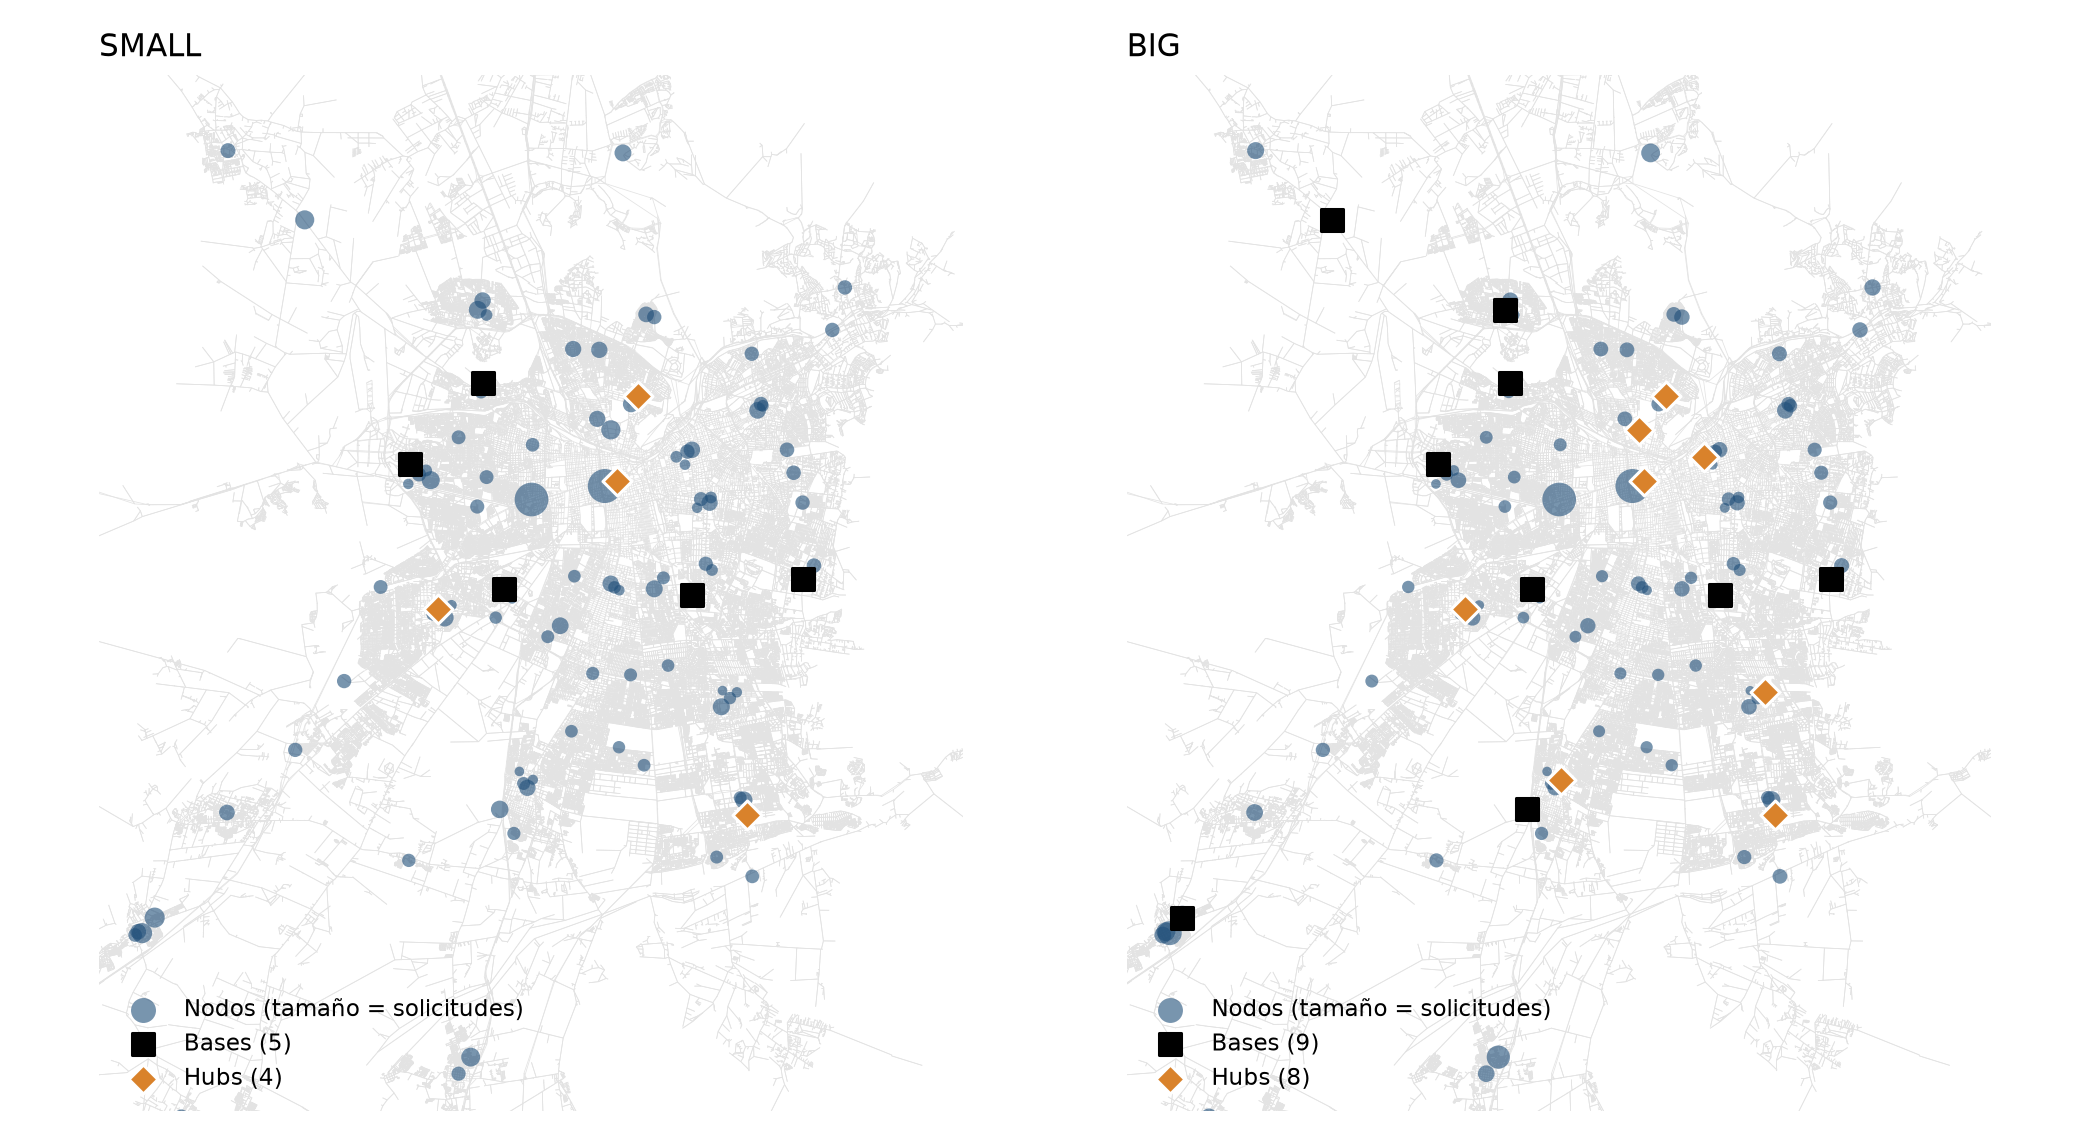
\includegraphics[width=0.92\textwidth]{figures/fig_mapa.png}
\caption{Establecimientos (tamaño según el número de solicitudes que los usan como origen o destino), bases y hubs disponibles en cada tamaño de instancia.}\label{fig:mapa}
\end{figure}

\parrafo{BIG no es solo más grande.} BIG tiene entre 1,8 y 2 veces las solicitudes de SMALL y exactamente el triple de flota, pero sus ventanas son mucho más estrechas: el 91\,\% de sus retiros tiene menos de 90 minutos para iniciarse, contra el 22\,\% en SMALL, y sus viajes son un 21\,\% más largos. La composición por clase, en cambio, es casi la misma: el insumo general es el 46,5\,\% de las solicitudes en SMALL y el 43,8\,\% en BIG, seguido por la muestra clínica (20,2 y 21,8\,\%), el equipo de retorno (19,2 y 20,1\,\%) y el fármaco refrigerado (14,1 y 14,3\,\%). La geografía es convergente: la demanda se reparte en la periferia, pero dos establecimientos del centro (Santiago Centro y Estación Central) concentran el 17,9\,\% de los destinos, lo que abre oportunidades de consolidar viajes hacia el centro.

\parrafo{La división es obligatoria, no opcional.} La Figura~\ref{fig:insumo} muestra que la distribución de cantidades del insumo general es bimodal. El 28,3\,\% de los insumos en SMALL y el 37,7\,\% en BIG supera las 70 unidades del furgón, el vehículo más grande, y por lo tanto solo se puede atender dividido o externalizado. Como el insumo es la única clase divisible, la división no es una mejora opcional sino una condición para no externalizar un tercio de los insumos.

\begin{figure}[htbp]
\centering
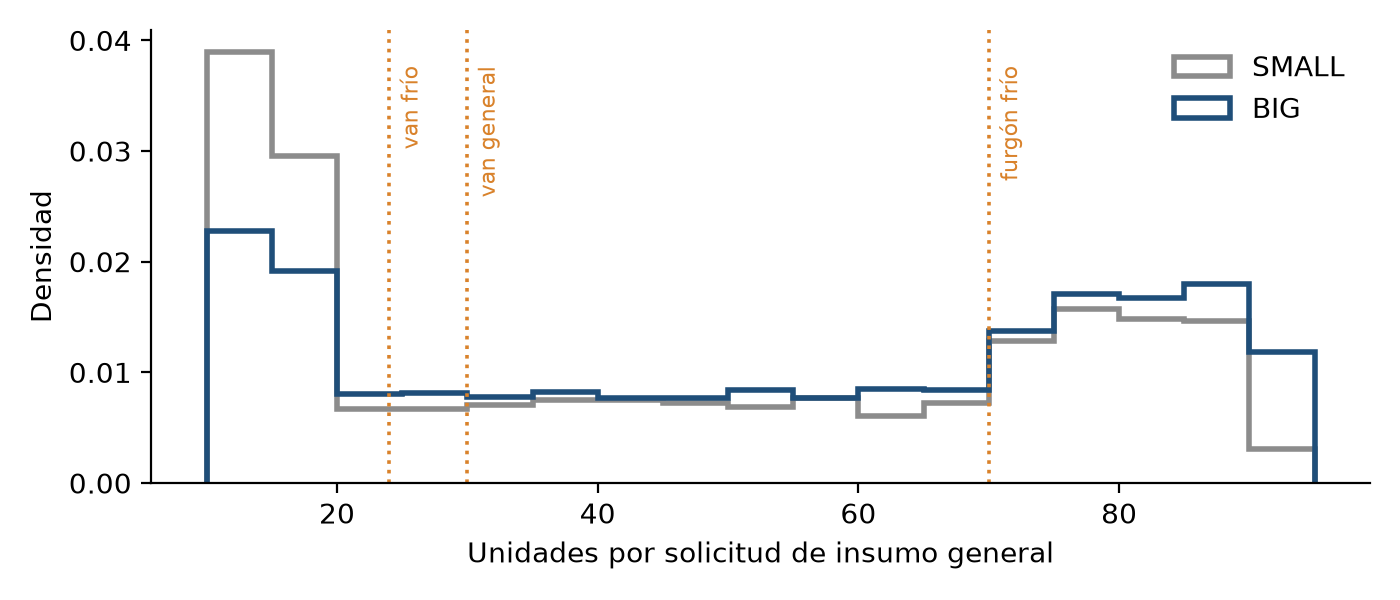
\includegraphics[width=0.72\textwidth]{figures/fig_insumo_capacidad.png}
\caption{Distribución de la cantidad de las solicitudes de insumo general y capacidad de cada tipo de vehículo.}\label{fig:insumo}
\end{figure}

\parrafo{Las ventanas concentran la demanda en pocas horas.} La Figura~\ref{fig:concurrencia} cuenta, cada 15 minutos, cuántas solicitudes están \emph{en curso}, es decir, ya abrieron su ventana de retiro y aún no vencen su entrega. Mientras están en curso, cada una necesita estar a bordo de algún vehículo o por ser recogida pronto. En lugar de un promedio, la figura muestra la mediana de los 200 días de cada tamaño y la banda entre los percentiles 10 y 90. En SMALL el máximo ocurre a las 14:45, con 34 solicitudes en curso en el día mediano y 48 en el peor, y supera la flota de 20 vehículos en los 200 días. En BIG el máximo se adelanta a las 10:00, cuando el día mediano iguala la flota de 60 vehículos y el peor llega a 97, y lo supera en el 70\,\% de los días. Como un vehículo puede llevar varias solicitudes a la vez, la flota alcanza, pero solo si las rutas consolidan bien en esas horas; por eso el costo depende tanto de la calidad del ruteo como del tamaño de la flota.

\begin{figure}[htbp]
\centering
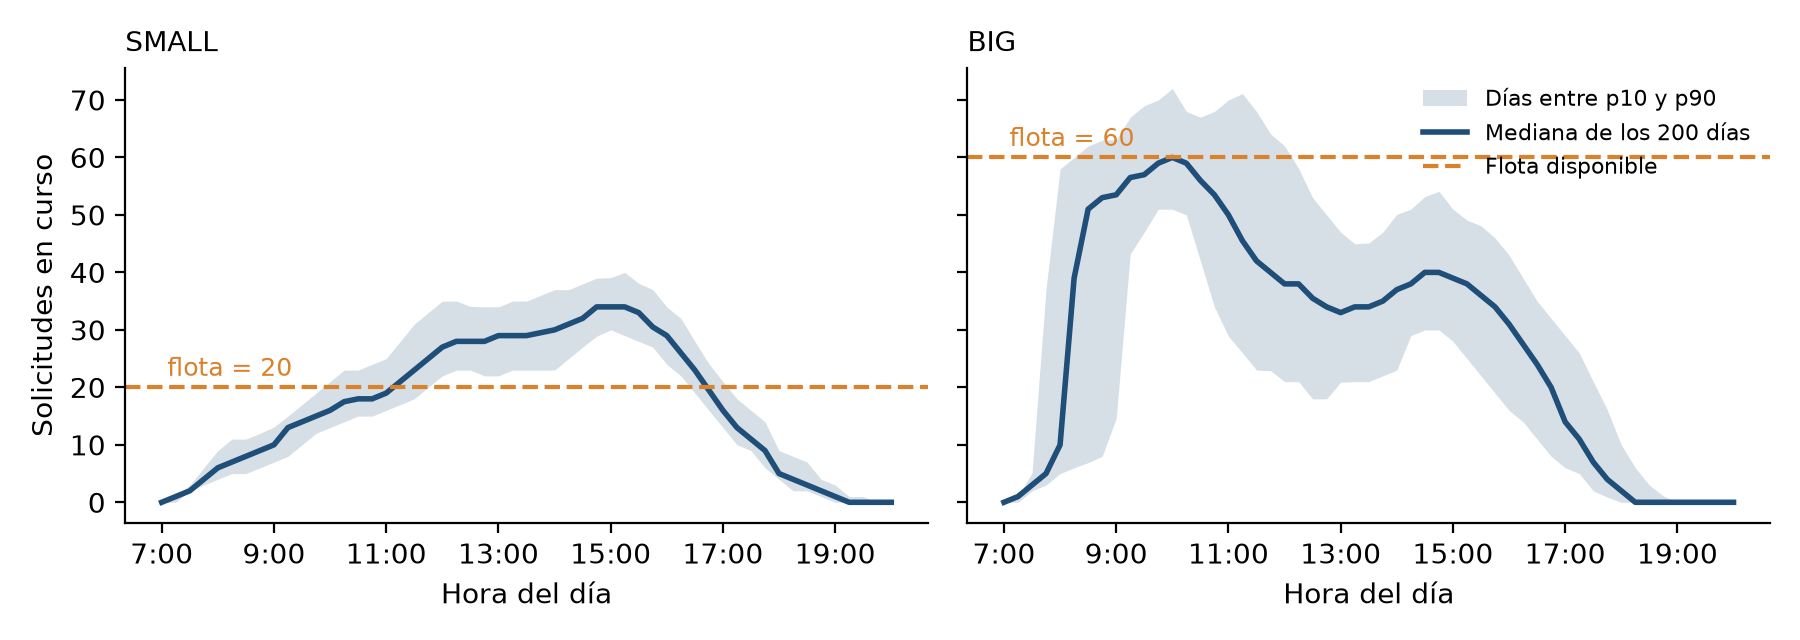
\includegraphics[width=0.92\textwidth]{figures/fig_concurrencia.png}
\caption{Solicitudes en curso a lo largo del día (entre la apertura de su retiro y el compromiso de su entrega), en los 200 días de cada tamaño de instancia.}\label{fig:concurrencia}
\end{figure}

\parrafo{El furgón es el recurso disputado.} El 34\,\% de las solicitudes en SMALL y el 36\,\% en BIG (muestras y fármacos) solo puede viajar en vehículos refrigerados, que son el 60\,\% de la flota. El furgón frío es el único vehículo compatible con las cuatro clases y el único que lleva insumos de más de 30 unidades sin dividir o equipos de más de 30 unidades, que son la mitad de los equipos. Es el más flexible, pero también el más caro de contratar y de operar: un furgón cuesta un 73\,\% más por semana que una van general y un 55\,\% más por kilómetro. Usarlo para cargas que caben en una van encarece la operación, mientras que reservarlo puede obligar a dividir o externalizar. Esa disyuntiva es una de las que la optimización tiene que resolver.

\parrafo{La incompatibilidad térmica limita la consolidación.} Se llama \emph{par expuesto} a una solicitud de fármaco y una de insumo del mismo día cuyos intervalos en curso se superponen, de modo que no pueden compartir vehículo en ese lapso. Hay en promedio 153 pares expuestos por día en SMALL y 503 en BIG. Como ambas clases pueden ir en vehículos refrigerados, esos pares obligan a separarlas justamente en los vehículos más disputados.

\section{Indicadores de desempeño}\label{sec:kpis}

La Tabla~\ref{tab:kpis} resume los indicadores con que se evalúan las soluciones. El costo total es el indicador principal y se reporta desglosado, porque un mismo total puede venir de estrategias muy distintas. Los demás indicadores explican de dónde viene el costo y verifican que una reducción no se logre a costa del servicio. Todos se calculan con el mismo código para el caso base y para la metodología propuesta.

\begin{table}[htbp]
\centering
\caption{Indicadores de desempeño y lo que permiten analizar.}\label{tab:kpis}
\small
\begin{tabularx}{\textwidth}{lYY}
\toprule
Área & Indicador y definición & Qué permite analizar \\
\midrule
Costo & Costo total semanal, desglosado en los bloques fijo, variable y de externalización; costo por solicitud. & Comparación económica global y origen del ahorro. \\
Servicio & Solicitudes externalizadas (número y \%); entregas atrasadas (\% de las atendidas). & Dependencia de terceros y cumplimiento de ventanas. \\
Recursos & Vehículos contratados por tipo; vehículo-días usados sobre vehículo-días pagados; fracción de la jornada usada; uso medio de la capacidad a bordo (carga media dividida por la capacidad, ponderada por kilómetro). & Tamaño y composición de la flota, capacidad ociosa. \\
Ruteo & Kilómetros por solicitud atendida; factor de recorrido (kilómetros recorridos divididos por la suma de las distancias origen--destino de las solicitudes atendidas); fracción de kilómetros en vacío; solicitudes por ruta. & Eficiencia de las rutas y nivel de consolidación. \\
\bottomrule
\end{tabularx}
\end{table}


\chapter[DISCUSIÓN METODOLÓGICA]{Discusión metodológica}\label{cap:metodologia}
\section{Revisión bibliográfica}\label{sec:revision}

\parrafo{Familia de problemas.} La operación diaria corresponde a un problema de recogida y entrega con ventanas de tiempo (PDPTW, por su sigla en inglés), en que cada solicitud une un origen con un destino y el retiro debe preceder a la entrega en el mismo vehículo \cite{parragh_doerner_hartl_2008}. La decisión semanal de qué bases usar y qué vehículos ubicar en ellas se asemeja a un problema de localización y ruteo (LRP) \cite{prodhon_prins_2014}. La externalización \cite{dabia_lai_vigo_2019} y la combinación de división de carga con transbordos \cite{wolfinger_salazar_2021} se han estudiado como extensiones, cada una por separado. En salud, el traslado de muestras entre centros se ha modelado como un problema de ruteo con ventanas y tiempos máximos de traslado \cite{benini_detti_zabalo_2021}, y la recolección domiciliaria de muestras, como un ruteo con capacidad y horarios \cite{ettazi_2021}.

\parrafo{Límites de los métodos exactos.} Los problemas de recogida y entrega son NP-difíciles porque generalizan el problema del vendedor viajero \cite{parragh_doerner_hartl_2008}: el tiempo que necesita un método exacto para probar optimalidad crece muy rápido con el número de solicitudes. En localización y ruteo, los métodos exactos resuelven de forma consistente instancias de unos 50 clientes y solo algunos casos de hasta 200 clientes con 10 a 14 depósitos; sobre ese tamaño dejan de cerrar la brecha de optimalidad en tiempos razonables \cite{prodhon_prins_2014}. Con flota propia y transportista externo, un algoritmo de ramificación y corte resolvió a optimalidad 272 de 504 instancias de hasta 100 clientes \cite{dabia_lai_vigo_2019}, y con división de carga y transbordos, el primer método exacto reportado resuelve instancias de 8 solicitudes, 3 puntos de transbordo y 2 a 3 vehículos \cite{wolfinger_salazar_2021}. Ninguno de esos trabajos combina todas las características a la vez.

\parrafo{Descomposición.} Para localización y ruteo, \citeA{prodhon_prins_2014} recogen que decidir primero la localización y después las rutas, sin volver atrás, conduce a soluciones subóptimas, y destacan los métodos que descomponen el problema pero iteran entre ambas partes intercambiando información.

\parrafo{Heurísticas de inserción y búsqueda local.} En el PDPTW, las heurísticas más usadas construyen rutas insertando pares retiro--entrega y luego las mejoran con movimientos que preservan el par; así se resolvió, por ejemplo, un PDPTW con transbordos mediante inserción más barata y mejora local (Mitrovi\'c-Mini\'c y Laporte, 2006, como se citó en \citeNP{parragh_doerner_hartl_2008}). GRASP \cite{feo_resende_1995} repite una construcción voraz aleatorizada y mejora cada resultado con búsqueda local; el descenso por vecindarios variables (VND) \cite{hansen_mladenovic_2001} aplica varios tipos de movimiento en orden hasta que ninguno mejora. Su combinación se ha usado en ruteo con camión y acoplado, donde el VND mejoró en promedio un 42\,\% las soluciones construidas \cite{villegas_2010}, y en recolección de residuos con ventanas y sincronización, con mejores resultados que un solver comercial en las instancias grandes \cite{perez_luis_2026}.

\parrafo{Matheurísticas y generación de columnas.} Una matheurística combina una heurística con un modelo de programación matemática \cite{archetti_speranza_2014}. Un esquema frecuente en ruteo con flota heterogénea es generar rutas con una heurística y elegir la mejor combinación con un modelo de particionamiento de conjuntos \cite{subramanian_2012,subramanian_2013}. La generación de columnas formaliza ese intercambio: un problema maestro elige entre las rutas conocidas y sus precios duales indican qué rutas nuevas podrían mejorarlo, que se buscan resolviendo un subproblema de \emph{pricing} \cite{desaulniers_2005}. Cuando el pricing se resuelve con una heurística, el método ya no prueba optimalidad, pero conserva la guía de los duales \cite{archetti_speranza_2014}.

\section{Alternativas metodológicas}\label{sec:alternativas}

La Tabla~\ref{tab:alternativas} resume las alternativas consideradas. Un modelo exacto con variables por arco necesita una variable por vehículo y par de puntos: el día SMALL más cargado tiene 77 solicitudes, es decir, 154 puntos de retiro y entrega más 9 bases y hubs, lo que da $163\cdot162\cdot20\approx 528$ mil variables binarias solo para el ruteo, y el día BIG más cargado, $325\cdot324\cdot60\approx 6{,}3$ millones. La parte semanal, en cambio, es pequeña: contratar cada vehículo, ubicarlo en cada base, abrir cada base y habilitar cada hub suma $20+20\cdot5+5+4=129$ variables binarias en SMALL y $60+60\cdot9+9+8=617$ en BIG. Esa diferencia de escala justifica tratar el ruteo con heurísticas y reservar el modelo exacto para la decisión semanal.

\begin{table}[htbp]
\centering
\caption{Alternativas metodológicas consideradas.}\label{tab:alternativas}
\small
\begin{tabularx}{\textwidth}{>{\raggedright\arraybackslash}p{3.6cm}YY}
\toprule
Alternativa & Ventajas & Desventajas \\
\midrule
MILP monolítico (ramificación y corte) & Óptimo y cota exacta; incorpora todas las restricciones. & No escala: millones de variables por día en BIG. \\
Búsqueda adaptativa de vecindario grande (ALNS) & Flexible ante restricciones nuevas; escala bien. & No decide bien la flota semanal; muchos operadores que calibrar. \\
GRASP + VND & Simple, rápida y siempre factible; buena diversidad. & Decide rutas día por día; no ve el costo fijo semanal. \\
Matheurística: rutas heurísticas + particionamiento de conjuntos con generación de columnas & Decide flota, bases, hubs y rutas en un mismo modelo; los duales guían la búsqueda; entrega una cota sobre las rutas generadas. & Más compleja de implementar; la cota no es del problema completo si el pricing es heurístico. \\
\bottomrule
\end{tabularx}
\end{table}

Se elige la matheurística porque es la única alternativa que compara en un mismo modelo el costo fijo de cada vehículo con los costos variables y de externalización que ese vehículo evita, que es justamente la disyuntiva que mostró el análisis de datos.

\section{Metodología propuesta}\label{sec:propuesta}

\parrafo{Conceptos.} La metodología trabaja con tres objetos:
\begin{itemize}\itemsep0pt
\item Un \textbf{tramo} es un par retiro--entrega que un solo vehículo hace completo. Una solicitud directa es un tramo; una dividida en dos partes son dos tramos del mismo origen al mismo destino; una transferida son dos tramos, del origen al hub y del hub al destino.
\item Un \textbf{plan} es una forma completa de atender una solicitud: el conjunto de tramos que la cubren. Cada solicitud tiene un plan directo y, si corresponde, planes de división y de transferencia.
\item Una \textbf{ruta} es el recorrido de un vehículo en un día: sale de su base, visita en orden los retiros y entregas de varios tramos y vuelve a su base. Cada ruta es factible por construcción: respeta capacidad, compatibilidad, incompatibilidad térmica, ventanas, tiempo máximo de traslado y jornada. En el modelo maestro, cada ruta es una \emph{columna}, es decir, una variable binaria que vale 1 si la ruta se usa.
\end{itemize}

\parrafo{Lógica general.} Un \emph{modelo maestro} semanal (un MILP de particionamiento de conjuntos resuelto con Gurobi) elige qué rutas usar entre las disponibles en un \emph{pool}, y con ello decide a la vez la flota, la base de cada vehículo, los hubs, el plan de cada solicitud y qué se externaliza. Las rutas del pool las generan dos heurísticas. GRASP + VND construye soluciones diarias completas y aporta un pool inicial diverso. Luego se resuelve la relajación lineal del maestro, cuyos precios duales indican cuánto vale cubrir cada tramo y cuánto cuesta usar cada vehículo cada día. Con esos precios, una heurística de \emph{pricing} construye rutas nuevas y agrega al pool solo las de \emph{costo reducido} negativo, es decir, las que pueden bajar el costo de la relajación. Esto se repite hasta que no aparecen rutas útiles; entonces se resuelve el maestro entero. La Figura~\ref{fig:flujo} muestra el flujo completo.

\begin{figure}[htbp]
\centering
\begin{tikzpicture}[
  caja/.style={draw, rounded corners=2pt, align=center, font=\footnotesize, minimum height=1.05cm, text width=2.9cm, fill=white},
  dec/.style={draw, diamond, aspect=2.3, align=center, font=\footnotesize, inner sep=0.5pt, fill=white},
  fl/.style={-{Stealth[length=2mm]}, thick}, et/.style={font=\scriptsize, align=center}]
\node[caja, fill=gray!12] (p1) at (0,0) {\textbf{1. Preparar}\\matriz de tiempos y planes};
\node[caja] (p2) at (3.65,0) {\textbf{2. GRASP + VND}\\pool inicial de rutas};
\node[caja] (p3a) at (7.3,0) {\textbf{3a. Relajación lineal}\\cota y precios duales};
\node[caja] (p3b) at (10.95,0) {\textbf{3b. Pricing}\\con los duales, rutas de costo reducido $<0$};
\node[caja] (p4) at (7.3,-2.3) {\textbf{4. Maestro entero}\\flota, bases, hubs, planes y rutas};
\node[caja] (p5) at (10.95,-2.3) {\textbf{5. Post-optimización}\\inserta externalizadas};
\node[dec] (d) at (10.95,-4.4) {¿quedan\\vueltas?};
\node[caja] (p6) at (3.65,-4.4) {\textbf{6. Reparar}\\planes de transferencia y división};
\node[caja, fill=gray!12] (p7) at (10.95,-6.3) {\textbf{7. Cerrar}\\mejor solución, KPIs y validación};
\draw[fl] (p1) -- (p2);
\draw[fl] (p2) -- (p3a);
\draw[fl] ([yshift=0.22cm]p3a.east) -- ([yshift=0.22cm]p3b.west);
\draw[fl] ([yshift=-0.22cm]p3b.west) -- ([yshift=-0.22cm]p3a.east);
\draw[fl] (p3a) -- node[et, right]{sin rutas nuevas\\o mejora $<$ 0,1\,\%} (p4);
\draw[fl] (p4) -- (p5);
\draw[fl] (p5) -- (d);
\draw[fl] (d) -- node[et, above]{sí} (p6);
\draw[fl] (p6) -- (p2);
\draw[fl] (d) -- node[et, right]{no (tras 3 vueltas)} (p7);
\end{tikzpicture}
\caption{Flujo de la matheurística para una semana. Los pasos 2 a 6 se repiten tres vueltas; el paso 7 toma la mejor solución encontrada.}\label{fig:flujo}
\end{figure}

\parrafo{Pasos.} (1) Una sola vez por semana se calcula la matriz de tiempos y distancias sobre la red vial y se arma el catálogo de planes: el directo de cada solicitud y, para las que exceden la capacidad de todo vehículo compatible, su división. Además, se resuelve el caso base del Capítulo~\ref{cap:casobase} y se mejoran sus rutas con el VND; esa solución entra al pool y sirve como punto de partida, de modo que la matheurística nunca entrega algo peor que la planificación por reglas. (2) GRASP + VND genera rutas para diez posicionamientos de la flota. La mitad de los arranques construye por arrepentimiento y la otra mitad en orden de urgencia (fin de la ventana de retiro); cada arranque usa una fracción sorteada, entre el 60 y el 100\,\%, de los vehículos de cada tipo, para que el pool contenga soluciones con flotas de distinto tamaño. (3) Se alternan la relajación lineal del maestro y el pricing, con un máximo de seis rondas, hasta que no aparecen rutas de costo reducido negativo o la cota mejora menos de 0,1\,\%. (4) El maestro entero elige la solución semanal partiendo de la mejor solución conocida, de modo que el costo nunca empeora entre vueltas. (5) Como el maestro solo combina rutas existentes, puede externalizar una solicitud aunque haya un vehículo pagado con tiempo libre; la post-optimización intenta insertar cada externalizada en las rutas de los vehículos ya contratados, la acepta si cuesta menos que externalizarla, y luego prueba contratar un vehículo adicional si el ahorro de la semana supera su costo fijo. El VND vuelve a acortar las rutas de la solución resultante. (6) Para las solicitudes que quedaron externalizadas o atrasadas se generan planes de transferencia y de división, que se prueban en la vuelta siguiente. (7) Tras tres vueltas se reporta la mejor solución y se valida cada restricción con un código independiente del que la generó.

\parrafo{Supuestos de modelación.} Los datos no especifican algunos elementos, que se fijaron como sigue:
\begin{itemize}\itemsep0pt
\item \textbf{Jornada} de 08:00 a 17:00, indicada por el ayudante. El retorno después de las 17:00 se paga como sobretiempo, con un máximo de 120 minutos por vehículo y día.
\item \textbf{Atraso} máximo de 180 minutos en las clases que lo admiten.
\item \textbf{Tiempos de viaje} fijos, calculados con la velocidad máxima de cada calle en la red vial (velocidad media resultante de 61,6 km/h, sin congestión). Es un supuesto optimista que se evalúa en el análisis de sensibilidad.
\item \textbf{Costo de externalización:} el de la hoja de clases (\$190.000 a \$250.000). La hoja de instancias trae exactamente el doble; se usó el primero por indicación del profesor y el segundo se evalúa como escenario.
\item \textbf{Documentación:} los documentos que exige cada clase no restringen la asignación, porque los datos no indican qué vehículo o conductor los porta.
\item \textbf{Personal} disponible en todos los establecimientos durante las ventanas de atención.
\end{itemize}


\chapter[CASO BASE]{Caso base}\label{cap:casobase}
El caso base representa cómo planificaría la semana un equipo que conoce todas las solicitudes con anticipación pero no usa optimización matemática: aplica reglas simples, de a una decisión por vez, y no vuelve atrás sobre lo ya decidido. Se usa como referencia para medir cuánto aporta coordinar las decisiones. Para que la comparación sea justa, el caso base usa los mismos datos, la misma matriz de tiempos, el mismo evaluador de rutas y el mismo validador que la metodología propuesta.

Respecto de la versión anterior, el caso base se corrigió en dos aspectos, a raíz de que externalizaba en promedio 33,6 solicitudes por semana, diez veces más que la matheurística. Un planificador que debe evitar externalizar no aceptaría ese resultado: revisaría su flota y aprovecharía mejor las rutas ya armadas. Las dos correcciones apuntan a eso y su efecto se cuantifica en la Sección~\ref{sec:resultados}.

\parrafo{Paso 1: flota inicial.} Se mantienen abiertas todas las bases. Cada solicitud se asocia a la base más cercana a su origen y se estima su carga de trabajo como el tiempo de ir desde la base al origen, atenderla, llevarla al destino y volver, como si se atendiera sola. Para cada tipo de vehículo se suma esa carga en el día más exigente de la semana y se divide por el 80\,\% de la jornada; el resultado es el número inicial de vehículos de ese tipo. Para cada solicitud se usa el tipo compatible más barato que la puede llevar. Los vehículos se reparten entre las bases en proporción a su carga estimada. El 80\,\% es solo un punto de partida, porque el paso 3 corrige la flota; su efecto se evalúa en la Sección~\ref{sec:sensibilidad}.

\parrafo{Paso 2: despacho diario.} Cada día, las solicitudes se ordenan por urgencia (primero las que cierran antes su ventana de retiro, luego las que no admiten atraso y luego las que vencen antes su entrega) y se procesan de a una. Cada solicitud se asigna al vehículo compatible que la puede incorporar sin atraso ni sobretiempo y al menor costo adicional. El vehículo la intercala en la mejor posición de su ruta ya armada, sin cambiar el orden de las paradas que ya tenía. En la versión anterior solo podía agregarla al final, lo que dejaba sin usar los huecos de la mañana. Si ningún vehículo puede hacerlo directamente, se prueban en orden la división, la transferencia por el hub más cercano al trayecto (pagando su costo fijo si aún no estaba habilitado) y la atención con atraso o sobretiempo. Se externaliza solo si ninguna de esas opciones es factible o si todas cuestan más que externalizar.

\parrafo{Paso 3: ajuste de la flota.} Este paso es nuevo. Terminada la semana, el planificador revisa las solicitudes externalizadas. Para cada una identifica el tipo de vehículo que la habría llevado y la base con cupo más cercana a su origen, y agrega un vehículo del par (tipo, base) que concentra más externalizaciones. Luego vuelve a despachar la semana completa. Si el costo total baja, conserva el vehículo y repite; si no, descarta ese par y prueba el siguiente. Se detiene cuando ningún vehículo adicional paga su costo fijo.

El Algoritmo~\ref{alg:base} resume el procedimiento y el Apéndice~\ref{ap:base} muestra un ejemplo.

\begin{algorithm}[htbp]
\caption{Caso base: planificación por reglas.}\label{alg:base}
\small
\KwIn{solicitudes de la semana, flota, bases y hubs}
\KwOut{flota contratada, base de cada vehículo, rutas diarias y externalizadas}
Abrir todas las bases; estimar la carga por base, tipo de vehículo y día\;
$F \leftarrow$ flota inicial al 80\,\% de la jornada en el día más exigente; repartirla entre bases\;
$S \leftarrow$ \textsc{Despachar}$(F)$; descartados $\leftarrow \emptyset$\;
\While{$S$ tiene externalizadas atendibles por un vehículo no contratado}{
  $(t,b) \leftarrow$ par (tipo, base) con más externalizadas, fuera de descartados\;
  $S' \leftarrow$ \textsc{Despachar}$(F \cup \{\text{un vehículo de tipo } t \text{ en } b\})$\;
  \lIf{\textup{costo}$(S') <$ \textup{costo}$(S)$}{$F \leftarrow F\cup\{\cdot\}$; $S\leftarrow S'$}
  \lElse{agregar $(t,b)$ a descartados}
}
\Return{$S$}\;
\BlankLine
\textsc{Despachar}$(F)$: para cada día, para cada solicitud en orden de urgencia: intercalar en el vehículo de $F$ factible más barato; si no hay, probar división, transferencia y atraso; si nada conviene, externalizar\;
\end{algorithm}

El caso base es razonable, porque usa información de la demanda, consolida solicitudes y revisa su flota. Sus límites son los de cualquier procedimiento secuencial: decide la flota con una estimación que ignora la consolidación, asigna cada solicitud mirando solo las que ya asignó, nunca reordena una ruta y agrega vehículos de a uno, sin reconsiderar dónde quedaron los anteriores.


\chapter[TRABAJO DESARROLLADO Y RESULTADOS]{Trabajo desarrollado y resultados}\label{cap:trabajo}
\section{Implementación}\label{sec:implementacion}

La herramienta está escrita en Python y usa Gurobi 13 para el modelo maestro. Cada semana se resuelve de forma independiente. El código está en el repositorio indicado en el Apéndice~\ref{ap:codigo}, y la Tabla~\ref{tab:modulos} relaciona cada módulo con la metodología.

\begin{table}[htbp]
\centering
\caption{Módulos del código y su papel en la metodología.}\label{tab:modulos}
\small
\begin{tabularx}{\textwidth}{lY}
\toprule
Módulo & Función \\
\midrule
\texttt{datos.py}, \texttt{matriz.py} & Leen los datos y calculan tiempos y distancias con un algoritmo de Dijkstra por origen sobre la red vial (paso 1). \\
\texttt{planes.py} & Genera los planes directos, de división y de transferencia, y sus tramos. \\
\texttt{ruta.py} & Evalúa una ruta: factibilidad completa, horarios y costo. \\
\texttt{heuristica.py} & GRASP + VND (paso 2) y pricing con duales (paso 3b). \\
\texttt{maestro.py} & Modelo maestro y su relajación lineal (pasos 3a y 4). \\
\texttt{completar.py} & Post-optimización por inserción (paso 5). \\
\texttt{validacion.py} & Revisa cada restricción de la solución final desde los datos originales (paso 7). \\
\texttt{caso\_base\_2.py} & Caso base del Capítulo~\ref{cap:casobase}. \\
\texttt{escenarios.py} & Escenarios del análisis de sensibilidad. \\
\texttt{analisis\_resultados.py} & Genera todas las tablas y figuras de resultados de este capítulo. \\
\bottomrule
\end{tabularx}
\end{table}

\parrafo{Entradas y salidas.} La herramienta recibe el archivo transversal, la hoja de solicitudes y la semana a resolver. Entrega, para esa semana, la flota contratada y la base de cada vehículo, los hubs habilitados, la forma de atención de cada solicitud, la secuencia y horario de cada ruta diaria, las solicitudes externalizadas, los indicadores de la Tabla~\ref{tab:kpis} y el informe de validación.

\parrafo{Parámetros.} En cada vuelta, GRASP + VND prueba 10 posicionamientos de la flota (la mitad reutiliza el de la mejor solución anterior) con una fracción sorteada de entre el 60 y el 100\,\% de cada tipo de vehículo. En la construcción por arrepentimiento, la lista restringida guarda las solicitudes cuyo arrepentimiento (la diferencia entre su segunda y su primera mejor inserción) es al menos el 85\,\% del máximo; en la construcción por urgencia, se elige al azar entre las tres solicitudes más urgentes. La entrega se intercala a lo más 8 posiciones después del retiro. El pool conserva hasta 300 rutas por vehículo y día. Los planes de transferencia consideran los 3 hubs con menor desvío y hasta 3 instantes de intercambio cada 30 minutos; en cada vuelta se reparan como máximo 125 solicitudes críticas. El maestro se detiene con una brecha de 1\,\% o tras 300 unidades de trabajo de Gurobi, un límite determinista que hace que dos corridas iguales entreguen la misma solución en cualquier computador.

\parrafo{Calibración.} Tres parámetros de la heurística se fijaron con un experimento sobre la semana 1 de la instancia 10, comparando la mejor solución inicial de cinco arranques (Tabla~\ref{tab:calibracion}). Penalizar la espera, como hacía la versión anterior (\$150 por minuto), empeoró las soluciones: evita rutas con tiempos muertos, pero obliga a usar más vehículos. Cobrar en la heurística la cuota diaria del costo fijo de cada vehículo ($f_k/5$) redujo la flota, pero alargó las rutas y subió el costo total en todas las combinaciones probadas, por lo que se dejó en cero: el costo fijo lo deciden el maestro, que lo paga completo, y el pricing, cuyos duales $\mu_{kd}$ lo incluyen. Sortear la fracción de la flota en cada arranque mejoró la construcción por urgencia.

\begin{table}[htbp]
\centering
\caption{Calibración de la heurística: mejor solución inicial de cinco arranques (instancia 10, semana 1).}\label{tab:calibracion}
\small
\begin{tabular}{lccccc}
\toprule
Construcción & Espera (\$/min) & Cuota fija & Flota & Costo (MM) & Vehículos \\
\midrule
Arrepentimiento (v1) & 150 & No & completa & 40,05 & 46 \\
Arrepentimiento & 150 & Sí & completa & 41,03 & 43 \\
Arrepentimiento & 50 & No & completa & 39,49 & 47 \\
Arrepentimiento & 50 & Sí & completa & 40,90 & 43 \\
Arrepentimiento & 0 & No & completa & 38,97 & 43 \\
Arrepentimiento & 0 & No & sorteada & 39,47 & 43 \\
Urgencia & 0 & No & completa & 40,62 & 44 \\
Urgencia & 0 & No & sorteada & 39,36 & 44 \\
\midrule
Caso base & -- & -- & -- & 38,87 & 34 \\
Caso base + VND & -- & -- & -- & 37,48 & 34 \\
\bottomrule
\end{tabular}
\end{table}

La última fila explica el diseño final. Ninguna construcción desde cero superó al caso base, que dimensiona una flota chica y la ajusta; pero sus rutas nunca se reordenan, y el VND las acorta un 3,6\,\%. Por eso la matheurística parte de esa solución y la usa como una columna más del pool.

\section{Modelo maestro y pricing}\label{sec:modelo}

\parrafo{Notación.} $R$ es el conjunto de solicitudes de la semana, $D$ el de días, $K$ el de vehículos, $B$ el de bases y $H$ el de hubs. $O_r$ es el conjunto de planes de la solicitud $r$, y $O^H\subseteq\bigcup_r O_r$ el de planes que pasan por un hub; $h(o)$ es el hub del plan $o$. $L$ es el conjunto de tramos y $L_o$ el de tramos del plan $o$. $\Omega_{kbd}$ es el conjunto de rutas del pool del vehículo $k$ saliendo de la base $b$ el día $d$, y $a_{\rho\ell}=1$ si la ruta $\rho$ hace el tramo $\ell$. Los costos son $f_k$ (fijo semanal del vehículo), $g_b$ (fijo de la base), $F_p$ (fijo del hub), $\pi_r$ (externalizar $r$), $c_o$ (manipulación en hub del plan $o$) y $c_\rho$ (costo de la ruta: kilómetros, sobretiempo y atraso). $\kappa_b$ es la capacidad de la base, y $\Gamma_p$ y $Q_p$ son las capacidades diarias del hub en operaciones y en unidades. Las variables binarias son $\lambda_\rho$ (se usa la ruta), $\xi_o$ (se usa el plan), $e_r$ (se externaliza), $y_k$ (se contrata el vehículo), $z_{kb}$ (el vehículo queda en la base), $u_b$ (se usa la base) y $h_p$ (se habilita el hub).

\begin{align}
\min\ & \sum_{k} f_k y_k + \sum_{b} g_b u_b + \sum_{p} F_p h_p + \sum_{r} \pi_r e_r + \sum_{o} c_o \xi_o + \sum_{\rho} c_\rho \lambda_\rho \label{eq:fo}\\
\text{s.a.}\ & \textstyle\sum_{o\in O_r} \xi_o + e_r = 1 && \forall r\in R \quad (\alpha_r) \label{eq:m1}\\
& \textstyle\sum_{\rho} a_{\rho\ell}\lambda_\rho = \sum_{o:\,\ell\in L_o} \xi_o && \forall \ell\in L \quad (\pi_\ell) \label{eq:m2}\\
& \textstyle\sum_{b}\sum_{\rho\in\Omega_{kbd}} \lambda_\rho \le y_k && \forall k\in K, d\in D \quad (\mu_{kd}) \label{eq:m3}\\
& \textstyle\sum_{\rho\in\Omega_{kbd}} \lambda_\rho \le z_{kb} && \forall k, b, d \quad (\nu_{kbd}) \label{eq:m4}\\
& \textstyle\sum_{b} z_{kb} = y_k,\quad z_{kb}\le u_b,\quad \sum_{k} z_{kb} \le \kappa_b u_b && \forall k, b \label{eq:m5}\\
& \xi_o \le h_{h(o)} \quad \forall o\in O^H; \qquad \textstyle\sum_{o\in O^H_{pd}} \xi_o \le \Gamma_p h_p,\ \ \sum_{o\in O^H_{pd}} q_o\xi_o \le Q_p h_p && \forall p, d \label{eq:m6}
\end{align}

La función objetivo \eqref{eq:fo} suma los tres bloques de costo de la Sección~\ref{cap:descripcion}. La restricción \eqref{eq:m1} atiende cada solicitud con un plan o la externaliza. La \eqref{eq:m2} es el vínculo entre planes y rutas: cada tramo de un plan elegido lo hace exactamente una ruta, y ningún tramo de un plan no elegido aparece en una ruta usada. La \eqref{eq:m3} permite a lo más una ruta por vehículo y día, y solo si el vehículo está contratado. La \eqref{eq:m4} obliga a que esa ruta salga de la base del vehículo. El grupo \eqref{eq:m5} asigna cada vehículo contratado a una sola base abierta y respeta su capacidad. El grupo \eqref{eq:m6} usa un plan con hub solo si el hub está habilitado y respeta su capacidad diaria, donde $O^H_{pd}$ son los planes que usan el hub $p$ el día $d$ y $q_o$ su cantidad. Las únicas restricciones que unen días distintos son las de diseño, a través de $y$, $z$, $u$ y $h$; por eso las rutas se pueden generar día por día.

\parrafo{Sincronización en los hubs.} Las transferencias no necesitan restricciones de tiempo en el maestro, porque la sincronización queda fijada dentro del plan. Cada plan de transferencia fija un hub y un instante de intercambio $\gamma$. El primer tramo debe terminar de descargar en el hub antes de $\gamma$ y el segundo puede cargar desde $\gamma$, por lo que el segundo vehículo nunca recoge antes de que el primero haya descargado. Además, el segundo tramo tiene un plazo absoluto que garantiza el tiempo máximo de traslado de origen a destino, que no se reinicia en el hub. La única aproximación es que $\gamma$ se toma en una grilla de 30 minutos, lo que puede descartar algunas transferencias, pero nunca genera una infactible.

\parrafo{Pricing.} Al resolver la relajación lineal se obtienen los duales $\alpha_r$, $\pi_\ell$, $\mu_{kd}\le0$ y $\nu_{kbd}\le0$ indicados en \eqref{eq:m1}--\eqref{eq:m4}. El \emph{costo reducido} de una ruta $\rho$ del vehículo $k$ desde la base $b$ el día $d$ es
\begin{equation}
\bar c_\rho = c_\rho - \sum_{\ell\in\rho} \pi_\ell - \mu_{kd} - \nu_{kbd}. \label{eq:cr}
\end{equation}
El término $\pi_\ell$ es cuánto vale para la relajación que se cubra el tramo $\ell$, y $-\mu_{kd}-\nu_{kbd}$ es cuánto cuesta usar ese vehículo ese día, incluida su parte del costo fijo. Solo las rutas con $\bar c_\rho<0$ pueden bajar el costo de la relajación. El pricing las busca con una inserción con premios. Para cada día y posicionamiento de la flota (el sugerido por la relajación y uno sorteado), inserta repetidamente el tramo y el vehículo de menor valor $\Delta c - \pi_\ell$, donde $\Delta c$ es el aumento del costo de la ruta, y suma el costo de usar el vehículo si la ruta estaba vacía. Se detiene cuando ningún valor es negativo. Cada tramo se usa una vez y, en cada solicitud, solo tramos de un mismo plan. Luego el VND acorta las rutas, y entran al pool las que tienen costo reducido negativo. Si un tramo aún no está en ninguna ruta del pool, no tiene dual propio; su precio se estima con el de su solicitud, $\alpha_r$ menos la manipulación del plan, repartido entre los tramos del plan según su cantidad.

\section{Coherencia entre el código y el informe}\label{sec:auditoria}

La corrección del Informe~2 señaló inconsistencias entre el código y su descripción. Se revisó el código línea por línea; la Tabla~\ref{tab:auditoria} resume lo encontrado y lo corregido. El cambio de mayor efecto fue el primero: el GRASP dejaba partes huérfanas de solicitudes divididas dentro de las rutas, y como el maestro no puede elegir una ruta que contiene un tramo de un plan incompleto, una sola parte huérfana inutilizaba la ruta completa. Con un solo arranque, en la instancia 10 semana 1, el maestro pasó de externalizar 378 de 599 solicitudes a externalizar 47.

\begin{table}[htbp]
\centering
\caption{Inconsistencias encontradas entre el código entregado y el Informe~2, y su corrección.}\label{tab:auditoria}
\footnotesize
\begin{tabularx}{\textwidth}{YY}
\toprule
Encontrado en la versión anterior & Corrección \\
\midrule
Partes huérfanas de divisiones inutilizaban rutas completas para el maestro. & Se sacan esas partes de las rutas antes de agregarlas al pool. \\
El informe describía generación de columnas, pero los duales se restaban a las dos mejores inserciones y se cancelaban en el arrepentimiento: no influían. & Pricing con costo reducido \eqref{eq:cr}; el GRASP queda como generador del pool inicial, sin duales. \\
La heurística no consideraba el costo fijo del vehículo. & Se agregó como opción (cuota $f_k/5$ al abrir un vehículo); empeoró el costo en todas las pruebas (Tabla~\ref{tab:calibracion}), así que el costo fijo lo manejan el maestro y los duales $\mu_{kd}$ del pricing. \\
El informe decía que todas las rutas visitadas entraban al pool. & Se describe lo que hace el código: entran las soluciones finales del GRASP y del VND de cada arranque y las rutas del pricing. \\
Reglas no declaradas: entrega a lo más 8 posiciones después del retiro y tope de 125 solicitudes críticas por vuelta. & Se declaran (Sección~\ref{sec:implementacion}) y quedan como parámetros. \\
El primer maestro no tenía punto de partida y, con un pool grande, terminaba con muchas externalizaciones. & La mejor solución entre el caso base mejorado con VND y el mejor arranque del GRASP es la solución inicial. \\
Todos los vehículos de un tipo se amontonaban en las mismas tres bases al sortear el posicionamiento. & Reparto proporcional a la demanda cercana a cada base, con azar. \\
Resultados irrepetibles sin fijar \texttt{PYTHONHASHSEED}, y dependientes de la velocidad del computador. & Recorridos en orden fijo y límite determinista de Gurobi. \\
La Tabla~3.2 mostraba un costo de externalización del doble del que usaba el código. & Se corrige (Tabla~\ref{tab:clases}); el doble se evalúa como escenario. \\
La directitud y las tablas de resultados no se generaban con el código entregado. & \texttt{analisis\_resultados.py} genera todas las tablas y figuras. \\
\bottomrule
\end{tabularx}
\end{table}

Además, la revisión del perfil de tiempo mostró que el 55\,\% del cómputo se iba en revisar la capacidad de rutas que luego se descartaban. Un filtro previo con el perfil de carga de la ruta redujo a menos de la mitad el tiempo del GRASP y del VND, sin cambiar ningún resultado. Finalmente, la solución del último maestro ahora también pasa por la post-optimización.

\section{Resultados}\label{sec:resultados}

Ambos métodos se corrieron en las 40 semanas BIG con los parámetros de la Sección~\ref{sec:implementacion}. La matheurística tardó en promedio 25 minutos por semana (máximo 44) usando dos hilos, y el caso base menos de un minuto. Todas las soluciones de ambos métodos pasaron la validación independiente: ninguna viola capacidad, compatibilidad, incompatibilidad térmica, ventanas, tiempo máximo de traslado, jornada, capacidad de bases ni capacidad de hubs.

\parrafo{Efecto de las correcciones.} La Tabla~\ref{tab:evolucion} compara las versiones del Informe~2 anterior con las actuales. El caso base corregido cuesta \$3,7 millones menos por semana que el anterior y externaliza 10 solicitudes en vez de 33,6. Eso hace la comparación más exigente: contra el caso base nuevo, la matheurística entregada antes habría ahorrado solo un 1,9\,\%. La matheurística corregida cuesta \$3,1 millones menos por semana que la anterior, con 8 vehículos menos y 4.100 kilómetros menos. Externaliza más que la versión anterior (7,2 contra 3,6 solicitudes), porque ya no contrata vehículos que solo se justifican para atender pocas solicitudes.

\begin{table}[htbp]
\centering
\caption{Promedio semanal en las 40 semanas BIG, antes y después de las correcciones.}\label{tab:evolucion}
\small
\begin{tabular}{lcccc}
\toprule
 & \multicolumn{2}{c}{Caso base} & \multicolumn{2}{c}{Matheurística} \\
\cmidrule(lr){2-3}\cmidrule(lr){4-5}
 & Anterior & Corregido & Anterior & Corregida \\
\midrule
Costo total (MM CLP) & 42,73 & 39,03 & 38,29 & 35,14 \\
Solicitudes externalizadas & 33,6 & 10,0 & 3,6 & 7,2 \\
Vehículos activados & 34,8 & 36,1 & 44,6 & 36,6 \\
Kilómetros & 31.960 & 32.841 & 31.598 & 27.455 \\
Alertas de la validación & -- & 0 & 31 & 6 \\
\bottomrule
\end{tabular}
\end{table}

\parrafo{Comparación global.} La matheurística es más barata que el caso base en las 40 semanas (Figura~\ref{fig:costosemanal}). El ahorro promedio es de 9,9\,\%, con un mínimo de 8,0\,\% y un máximo de 12,9\,\%, lo que equivale a \$3,9 millones por semana o unos \$200 millones al año si la demanda mantiene este patrón. El ahorro no depende de una semana en particular: va de 8,8 a 12,0\,\% entre instancias (Tabla~\ref{tab:instancias}) y no se correlaciona con cuánto externaliza el caso base ($r=-0{,}01$). Es decir, no viene de corregir semanas en que el caso base falla, sino de rutear mejor en todas.

\begin{figure}[htbp]
\centering
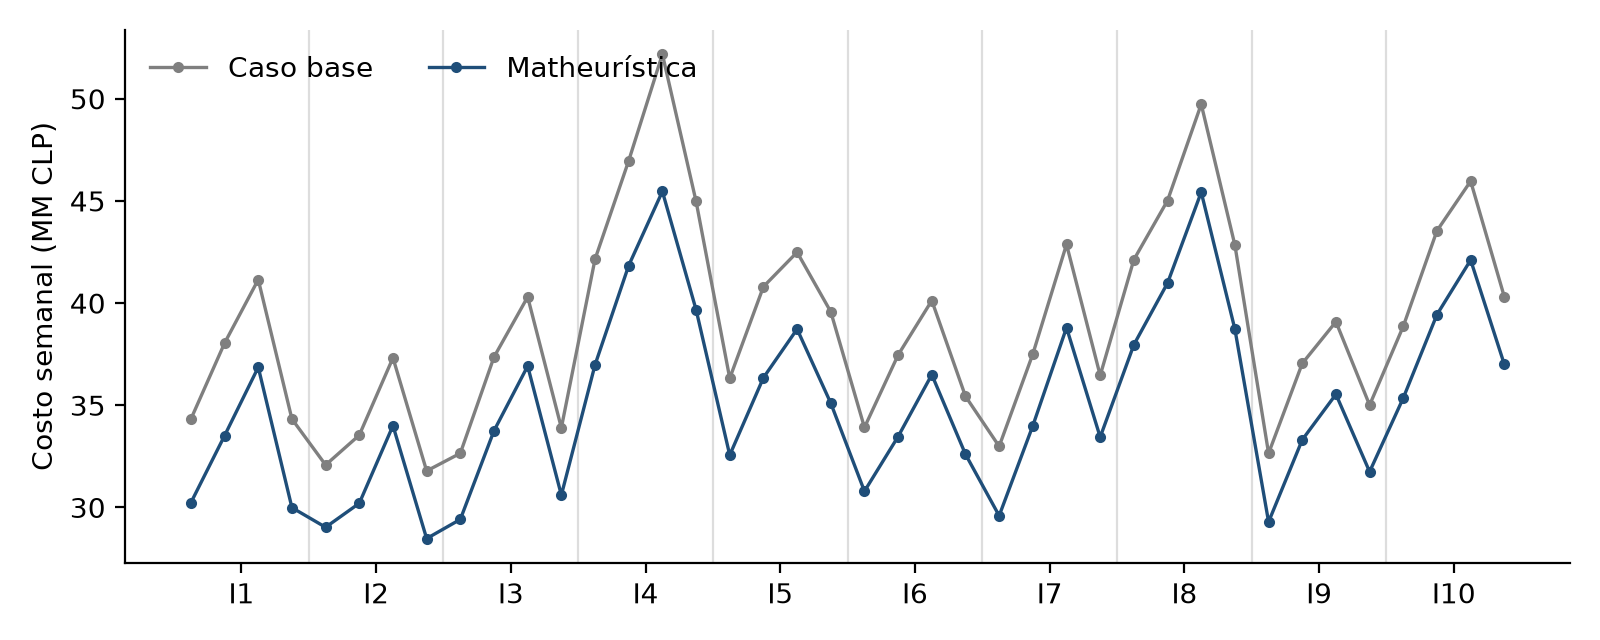
\includegraphics[width=\textwidth]{figures/fig_costo_semanal.png}
\caption{Costo semanal de ambos métodos en las 40 semanas BIG (cuatro semanas por instancia).}\label{fig:costosemanal}
\end{figure}

\begin{table}[htbp]
\centering
\caption{Resultados por instancia (promedio de sus cuatro semanas). Vehículos y externalizadas: caso base / matheurística.}\label{tab:instancias}
\small
\begin{tabular}{ccccccc}
\toprule
Instancia & Solicitudes & \multicolumn{2}{c}{Costo (MM CLP)} & Ahorro & Vehículos & Externalizadas \\
\cmidrule(lr){3-4}
 & por semana & Base & Matheur. & & & \\
\midrule
\tabinput{tablas/instancias.tex}
\bottomrule
\end{tabular}
\end{table}

\parrafo{De dónde viene el ahorro.} La Tabla~\ref{tab:desglose} desglosa el costo. Los kilómetros explican el 84\,\% del ahorro (\$3,26 de \$3,88 millones) y la externalización el 15\,\%; el costo fijo de vehículos sube levemente. La Tabla~\ref{tab:kpisres} muestra el mecanismo. Con casi la misma flota, la matheurística recorre un 16\,\% menos: el factor de recorrido baja de 2,10 a 1,74, es decir, por cada kilómetro que separa el origen y el destino de una solicitud se recorren 1,74 kilómetros en vez de 2,10. Las rutas consolidan más (4,25 tramos por ruta contra 3,99), los vehículos viajan más llenos (40\,\% de uso medio de capacidad contra 36,6\,\%) y recorren menos kilómetros vacíos. El caso base solo agrega cada solicitud a una ruta ya armada sin reordenarla, mientras que el VND y el maestro reordenan y recombinan rutas completas.

\begin{table}[htbp]
\centering
\caption{Desglose del costo semanal promedio (MM CLP).}\label{tab:desglose}
\small
\begin{tabular}{lccccc}
\toprule
Componente & Caso base & \% & Matheurística & \% & Diferencia \\
\midrule
\tabinput{tablas/desglose.tex}
\bottomrule
\end{tabular}
\end{table}

\begin{table}[htbp]
\centering
\caption{Indicadores de desempeño, promedio de las 40 semanas BIG. Los indicadores en porcentaje se comparan en puntos porcentuales (pp).}\label{tab:kpisres}
\small
\begin{tabular}{lccc}
\toprule
Indicador & Caso base & Matheurística & Cambio \\
\midrule
\tabinput{tablas/kpis.tex}
\bottomrule
\end{tabular}
\end{table}

\parrafo{Lo que empeora.} Las entregas atrasadas suben de 0,23 a 0,71\,\% (de 1,3 a 4,1 entregas por semana). Solo se atrasan insumos y equipos, que lo admiten, y el costo total de atraso es el mismo en ambos métodos (\$0,04 millones), porque la penalización por minuto (\$800 y \$1.200) es baja frente al costo de un desvío. Si la organización valora más la puntualidad que lo que indican esas penalizaciones, puede prohibir el atraso: la Sección~\ref{sec:sensres} muestra que hacerlo deja las entregas atrasadas en cero sin subir el costo. Además, el 7,9\,\% de los vehículo-días pagados quedan sin salir (contra 0,4\,\% en el caso base): la matheurística contrata vehículos que se necesitan en los días de mayor demanda y que quedan ociosos el resto de la semana, porque el costo fijo es semanal.

\parrafo{Flota y bases.} Ambos métodos contratan cerca de 8 vans generales, 11,5 vans frías y 17,3 furgones fríos por semana, de 24, 18 y 18 disponibles. El furgón es el recurso escaso: en 26 de las 40 semanas ambos métodos usan los 18, y en esas semanas la matheurística externaliza en promedio 8,3 solicitudes, contra 5,0 en las demás. Es el único vehículo que lleva insumos de más de 30 unidades sin dividirlos, equipos de más de 30 unidades y las cuatro clases a la vez. Ambos métodos usan las 9 bases casi todas las semanas, y la matheurística reparte los vehículos de forma parecida al caso base: mueve medio vehículo hacia Cerrillos y Pudahuel, en el poniente, y lo saca de Quilicura y Macul (Figura~\ref{fig:bases}). Aunque en total se usan unos 37 de los 62 cupos, algunas bases se llenan: Macul y Talagante quedan al tope en 23 de las 40 semanas y Cerrillos en 8. Los hubs casi no se usan (0,4 transferencias por semana): con tiempos de flujo libre, el desvío hacia un hub y la espera del intercambio rara vez convienen frente a una ruta directa. El escenario de hubs para todas las solicitudes (Sección~\ref{sec:sensres}) confirma que no se debe a la forma en que se generan los planes.

\begin{figure}[htbp]
\centering
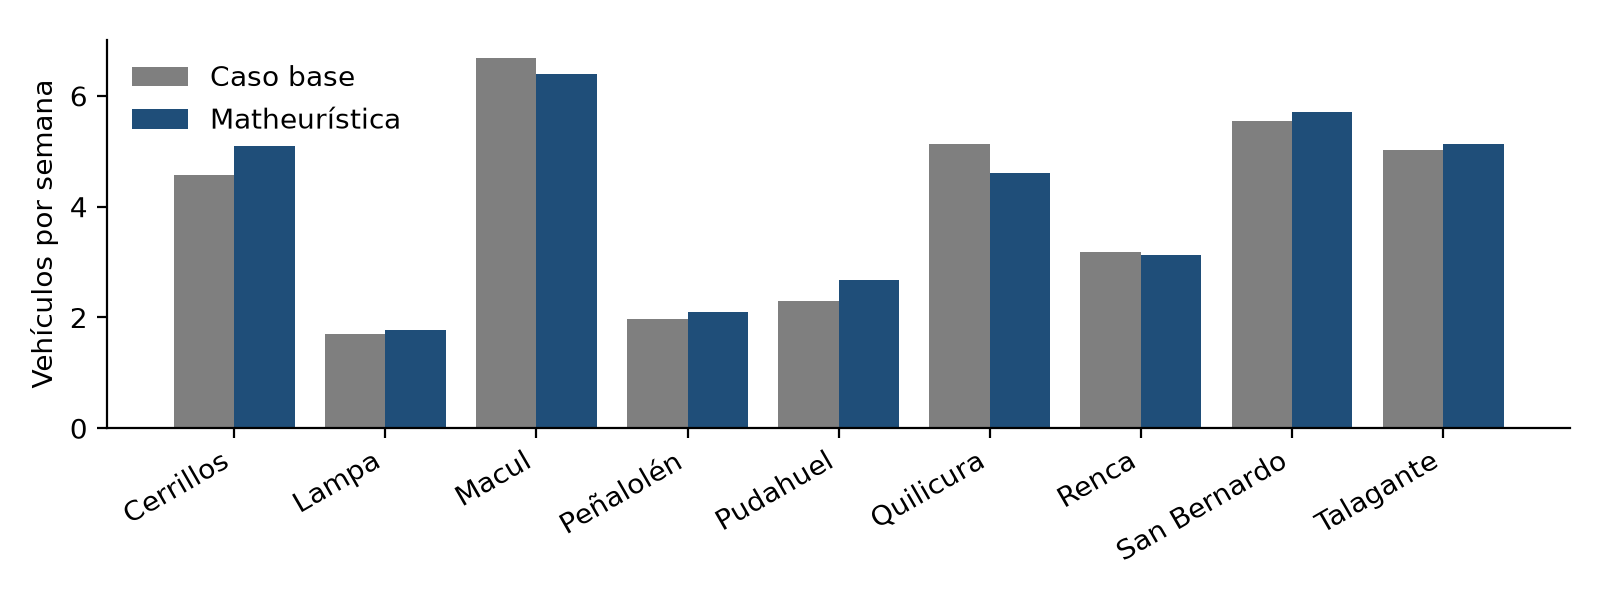
\includegraphics[width=0.9\textwidth]{figures/fig_bases.png}
\caption{Vehículos asignados a cada base, promedio de las 40 semanas.}\label{fig:bases}
\end{figure}

\parrafo{Solicitudes difíciles (objetivo O2).} De las 287 solicitudes que la matheurística externaliza en las 40 semanas, 253 también las externaliza el caso base, lo que indica que la dificultad es de la solicitud y no del método. Tienen un perfil claro: el 64\,\% son insumos y el 35\,\% equipos de retorno; su cantidad media es de 68,5 unidades, contra 32,1 del total; el 99\,\% tiene una ventana de retiro de una hora o menos, y el 40\,\% abre su retiro antes de las 09:00. Son solicitudes que necesitan un furgón o dos vehículos a la vez en un intervalo corto, justo cuando la flota de furgones está ocupada. Las de insumo son además las más baratas de externalizar (\$190.000), por lo que el modelo las elige primero cuando la capacidad no alcanza.

\parrafo{Aporte de la generación de columnas.} En la primera vuelta, el VND sobre la solución del caso base ahorra en promedio un 5,9\,\%; las vueltas siguientes, con generación de columnas, maestro y post-optimización, llevan el ahorro al 9,9\,\%. En cada semana se hacen entre 10 y 16 rondas de pricing, que agregan en promedio 2.450 rutas de costo reducido negativo a un pool final de unas 18.100. Esas rutas bajan la cota de la relajación lineal un 14\,\% respecto de la obtenida solo con las rutas del GRASP. La brecha entre la solución final y esa cota es de 10,7\,\% en promedio (8,1 a 12,8\,\%), contra 15,1\,\% en la versión anterior. Como el pricing es heurístico, la cota vale para el pool generado y no para el problema completo: indica que el maestro aprovecha bien las rutas disponibles, no que la solución esté a menos de 10,7\,\% del óptimo.

\parrafo{Validación.} Además de verificar la factibilidad, el validador revisa la coherencia económica de cada solución. En 35 de las 40 semanas no hay ninguna alerta. En las otras cinco hay seis: insumos de más de 70 unidades externalizados aunque había vehículos pagados sin salir ese día. Atenderlos exige dividirlos entre dos o tres de esos vehículos en la misma ventana de una hora, combinación que la post-optimización, que inserta un tramo a la vez, no prueba. Es una mejora pendiente acotada: valdría a lo más \$1,1 millones en total en las 40 semanas.

\section{Escalabilidad: instancias SMALL}\label{sec:small}

Para evaluar cómo se comporta el método en otro tamaño de red (objetivo O5), ambos métodos se corrieron en las 40 semanas SMALL con los mismos parámetros que en BIG. SMALL tiene la mitad de las solicitudes, un tercio de la flota (20 vehículos) y cinco bases, pero ventanas mucho más holgadas (Sección~\ref{sec:datos}). Todas las soluciones pasaron la validación independiente.

\parrafo{El ahorro es mayor en SMALL.} La matheurística es más barata que el caso base en las 40 semanas, con un ahorro promedio de 15,7\,\% (entre 11,6 y 19,5\,\%), equivalente a \$2,7 millones por semana (Tabla~\ref{tab:small}). El mecanismo es el mismo que en BIG: con la misma flota (15,8 vehículos en promedio en ambos métodos) recorre un 17\,\% menos de kilómetros. La diferencia de magnitud se explica por las ventanas. En SMALL solo el 22\,\% de los retiros tiene menos de 90 minutos para iniciarse, contra el 91\,\% en BIG, de modo que el VND y el maestro tienen mucho más espacio para reordenar y consolidar paradas. El caso base, que inserta cada solicitud en la ruta ya armada sin reordenarla, no aprovecha esa holgura. La externalización es baja en ambos métodos (2,4 y 1,8 solicitudes por semana) y se concentra en la instancia 8, la de más insumos grandes.

\begin{table}[htbp]
\centering
\caption{Resultados por instancia SMALL (promedio de sus cuatro semanas). Vehículos y externalizadas: caso base / matheurística.}\label{tab:small}
\small
\begin{tabular}{ccccccc}
\toprule
Instancia & Solicitudes & \multicolumn{2}{c}{Costo (MM CLP)} & Ahorro & Vehículos & Externalizadas \\
\cmidrule(lr){3-4}
 & por semana & Base & Matheur. & & & \\
\midrule
\tabinput{tablas/small_instancias.tex}
\bottomrule
\end{tabular}
\end{table}

\parrafo{Esfuerzo computacional.} La Tabla~\ref{tab:escala} compara ambos tamaños. Pasar de SMALL a BIG duplica las solicitudes y triplica la flota, pero el tiempo mediano por semana sube solo de 15,6 a 24,5 minutos y el pool final de 7.156 a 18.097 rutas. El crecimiento es moderado porque el maestro se detiene por un límite de trabajo y porque el pool se acota a 300 rutas por vehículo y día. En ambos tamaños, la generación de rutas con GRASP + VND consume más del 70\,\% del tiempo, el maestro entre 16 y 27\,\% y el pricing el resto; el cuello de botella computacional es, por lo tanto, la heurística y no Gurobi. Los tiempos de SMALL se midieron en los computadores de los integrantes del grupo, que no son idénticos, por lo que sirven como orden de magnitud. Las soluciones, en cambio, no dependen del computador, porque el límite de trabajo de Gurobi es determinista.

\begin{table}[htbp]
\centering
\caption{Comparación del método entre las 40 semanas SMALL y las 40 semanas BIG (promedios salvo indicación).}\label{tab:escala}
\small
\begin{tabular}{lcc}
\toprule
Indicador & SMALL & BIG \\
\midrule
\tabinput{tablas/escala.tex}
\bottomrule
\end{tabular}
\end{table}

\parrafo{Estrategias para redes más grandes.} Como cada día se construye por separado, la generación de rutas puede repartirse entre procesadores, día por día, sin cambiar el resultado; con cinco días, esto reduciría el tiempo de la fase más cara a cerca de un quinto. El tamaño del maestro se controla con el tope de rutas por vehículo y día y con el límite de trabajo. Si la red creciera mucho más, la descomposición natural es geográfica: resolver por separado zonas con sus bases y coordinar en el maestro solo los vehículos que cruzan zonas.

\section{Variabilidad y calidad de la solución}\label{sec:calidad}

\parrafo{El ahorro es estadísticamente significativo.} Como ambos métodos se aplican a las mismas semanas, la comparación es pareada: para cada semana se calcula el ahorro porcentual de la matheurística respecto del caso base. La Tabla~\ref{tab:estadistica} resume esos 40 ahorros por tamaño. El intervalo de confianza de 95\,\% para el ahorro medio es de 9,5 a 10,3\,\% en BIG y de 15,0 a 16,4\,\% en SMALL. Como el ahorro no tiene por qué distribuirse en forma normal, se aplica también la prueba de rangos con signo de Wilcoxon, que no supone una distribución: como las 40 semanas tienen ahorro positivo, la probabilidad de observar ese resultado si ambos métodos fueran equivalentes es menor que $10^{-12}$ en cada tamaño. La ventaja del método no se explica por azar.

\begin{table}[htbp]
\centering
\caption{Prueba pareada del ahorro de la matheurística frente al caso base. IC: intervalo de confianza de 95\,\% (t de Student, 39 grados de libertad). Valor $p$: prueba de Wilcoxon de una cola.}\label{tab:estadistica}
\small
\begin{tabular}{lcccccc}
\toprule
Tamaño & Semanas & Ahorro medio & IC 95\,\% (\%) & Estadístico $t$ & Semanas con ahorro & Valor $p$ \\
\midrule
\tabinput{tablas/estadistica.tex}
\bottomrule
\end{tabular}
\end{table}

\parrafo{Variabilidad por la semilla.} La matheurística es aleatoria: GRASP sortea la construcción y la fracción de la flota de cada arranque. Para medir cuánto depende el resultado de la semilla, cuatro semanas BIG que cubren el rango de demanda (455, 589, 692 y 731 solicitudes) se resolvieron con tres semillas adicionales a la original (Tabla~\ref{tab:semillas}). El coeficiente de variación del costo es como máximo 0,64\,\%, y el peor ahorro obtenido con cualquier semilla sigue siendo de 8,2\,\% o más. La variación entre semillas es entre 20 y 770 veces menor que la diferencia con el caso base, por lo que una sola corrida por semana basta para comparar. La variabilidad es mayor en la semana de menor demanda (instancia 1, semana 1), donde hay más formas de armar rutas de costo parecido y, por lo tanto, más soluciones distintas cercanas.

\begin{table}[htbp]
\centering
\caption{Costo de la matheurística con cuatro semillas (MM CLP). DE: desviación estándar; CV: coeficiente de variación.}\label{tab:semillas}
\small
\setlength{\tabcolsep}{4pt}
\begin{tabular}{cccccccccc}
\toprule
Instancia & Semana & Caso base & Original & Semilla 1 & Semilla 2 & Semilla 3 & DE & CV & Ahorro \\
\midrule
\tabinput{tablas/semillas.tex}
\bottomrule
\end{tabular}
\end{table}

\parrafo{La solución es aproximada.} La matheurística no prueba optimalidad, por tres razones: el pricing es heurístico, el maestro entero se detiene por un límite de trabajo y la post-optimización solo inserta un tramo a la vez. La única cota disponible es la relajación lineal del maestro sobre el pool final, y la brecha contra ella es de 10,7\,\% en BIG y 7,5\,\% en SMALL. Esa cota vale para las rutas generadas y no para el problema completo, de modo que no permite afirmar que la solución esté a menos de esa distancia del óptimo. Lo que sí muestra es que el pricing aporta: las rutas que agrega bajan la cota un 14\,\% en BIG y un 11\,\% en SMALL respecto de la obtenida solo con GRASP, es decir, encuentra combinaciones que la heurística sola no veía. Obtener una cota válida para el problema completo exigiría resolver el pricing de forma exacta, un problema de ruteo con todas las restricciones del caso que, como se discutió en la Sección~\ref{sec:revision}, los métodos exactos no resuelven en el tamaño de BIG.



\chapter[ANÁLISIS DE SENSIBILIDAD]{Análisis de sensibilidad}\label{cap:sensibilidad}
La sensibilidad busca responder dos preguntas: si la ventaja de coordinar se mantiene cuando cambian los supuestos, y cómo cambia la estructura de la solución (flota, bases, externalización) cuando cambian la demanda, la oferta y los costos (objetivo O3). Las alternativas de infraestructura, como cerrar o abrir bases y agregar furgones, se analizan en el Capítulo~\ref{cap:implementacion}.

\section{Escenarios y su justificación}\label{sec:sensibilidad}

Cada escenario modifica un solo elemento respecto de los datos originales y se resuelve con ambos métodos y los mismos parámetros de la Sección~\ref{sec:implementacion}. Los parámetros se eligieron por una de tres razones: son un supuesto incierto del modelo (tiempos de viaje, costo de externalizar), representan algo que la organización no controla (demanda, disponibilidad de flota) o son una decisión que podría tomar (jornada, ventanas, exigencia de puntualidad, uso de hubs y de la división). La Tabla~\ref{tab:escenarios} detalla cada uno.

Para controlar el cómputo, los escenarios principales se resolvieron en cuatro semanas que cubren el rango de demanda: la de menor demanda (instancia 1, semana 1, 455 solicitudes), la mediana (instancia 7, semana 4, 589), una exigente con muchas externalizaciones (instancia 8, semana 3, 692) y la de mayor demanda (instancia 10, semana 3, 731). Los rangos intermedios y los escenarios nuevos se resolvieron en las semanas mediana y de mayor demanda. En total son 60 corridas de la matheurística, cada una con su caso base.

\begin{table}[htbp]
\centering
\caption{Escenarios de sensibilidad y su justificación.}\label{tab:escenarios}
\footnotesize
\begin{tabularx}{\textwidth}{lYY}
\toprule
Escenario & Cambio & Por qué \\
\midrule
Demanda $-20$ a $+30$\,\% & Se agregan copias o se eliminan al azar solicitudes de cada día. & La demanda semanal varía entre 455 y 731 solicitudes; mide cuánta holgura tiene la red y si la flota crece en proporción. \\
Flota $-25$\,\% & Se retira un cuarto de los vehículos de cada tipo. & Vehículos en mantención o contratos no renovados: dónde aparece primero la escasez. \\
Congestión $+15$ a $+50$\,\% & Todos los tiempos de viaje se alargan. & Los tiempos de la red vial suponen flujo libre (61,6 km/h); es el supuesto más optimista del modelo. \\
Ventanas $+30$ y $-15$ min & Se mueve el cierre de cada ventana de retiro y de entrega. & Los centros podrían flexibilizar sus horarios o exigir más; el 99\,\% de las solicitudes difíciles tiene ventanas de una hora o menos. \\
Jornada desde las 07:00 & La jornada regular parte una hora antes. & En BIG, unas 13 solicitudes diarias abren su retiro antes de las 08:00; mide el valor de adelantar turnos. \\
Sin atraso permitido & Ninguna clase admite atraso. & La matheurística atrasa más entregas que el caso base; mide cuánto cuesta exigir puntualidad total. \\
Externalización $\times2$ y $\times0{,}5$ & Cambia el costo por solicitud externalizada. & El dato es ambiguo (la hoja de instancias trae el doble) y es el precio que compite con contratar vehículos. \\
Bases: costo fijo $\times2$ & Se duplica el costo semanal de las bases. & Mide si conviene concentrar la flota en menos bases. \\
Bases: capacidad $+50$ y $-25$\,\% & Cambia el número de vehículos que admite cada base. & Macul y Talagante quedan llenas en 23 de las 40 semanas; mide si su capacidad limita. \\
Hubs para todas & Planes de transferencia para todas las solicitudes transferibles. & Los hubs casi no se usan; mide si es por la forma de generar los planes (objetivo O5). \\
Sin división & Ninguna solicitud se puede dividir. & Mide el valor de la división, la otra forma de coordinación (objetivo O5). \\
Utilización del caso base & 60 a 100\,\% en vez de 80\,\%, en las 40 semanas. & Verifica que la comparación no dependa de ese parámetro del caso base. \\
\bottomrule
\end{tabularx}
\end{table}

\section{Resultados}\label{sec:sensres}

\begin{table}[htbp]
\centering
\caption{Resumen de la sensibilidad. Cambio de costo de la matheurística respecto de los datos originales de la misma semana, ahorro frente al caso base en el escenario y cambio medio en las solicitudes externalizadas por la matheurística. El detalle por semana está en el Apéndice~\ref{ap:sensibilidad}.}\label{tab:sensibilidad}
\footnotesize
\begin{tabular}{lcccc}
\toprule
Escenario & Semanas & Cambio de costo & Ahorro frente al caso base & Cambio en externalizadas \\
\midrule
\tabinput{tablas/sens_resumen.tex}
\bottomrule
\end{tabular}
\end{table}

\parrafo{La ventaja se mantiene.} La Tabla~\ref{tab:sensibilidad} resume las corridas, todas validadas sin errores. La matheurística es más barata que el caso base en todos los escenarios y semanas, con ahorros entre 5,0 y 14,0\,\%. Ningún supuesto evaluado hace desaparecer el beneficio de coordinar. Los ahorros más bajos aparecen cuando hay mucha externalización (sin división, con más demanda o con externalización barata): esa parte del costo la pagan casi por igual ambos métodos y queda menos ruteo que optimizar.

\begin{figure}[htbp]
\centering
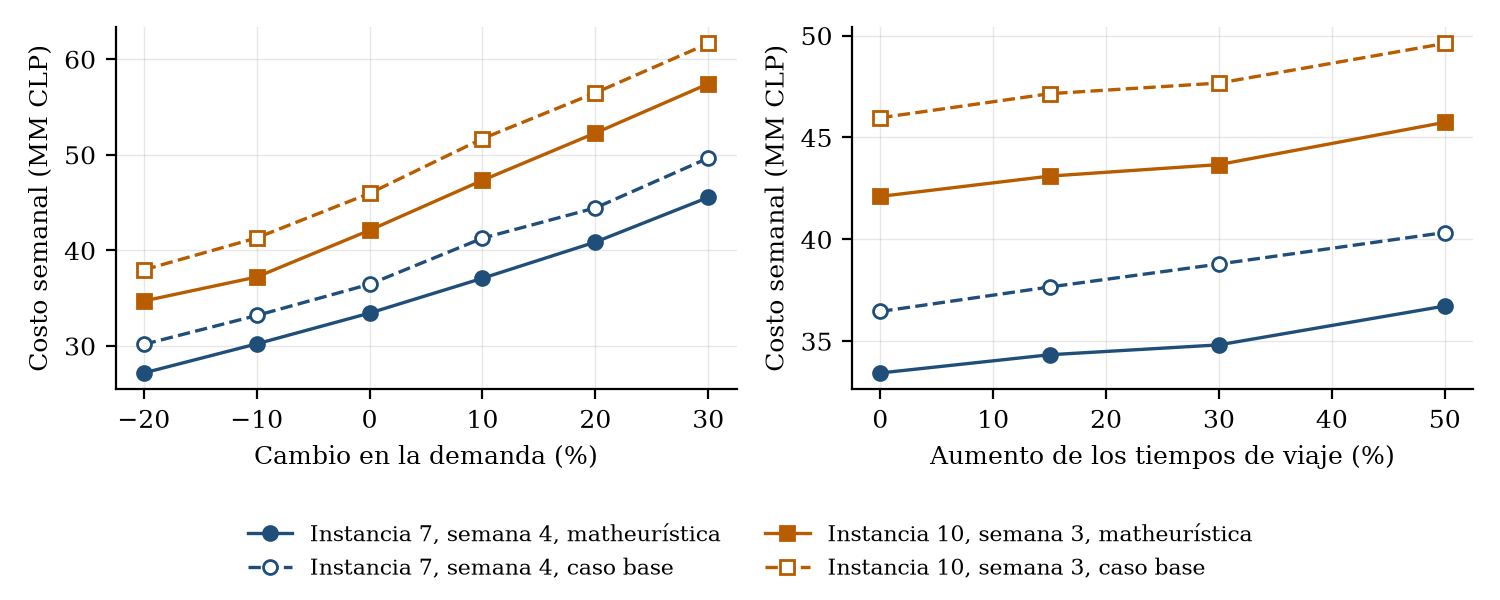
\includegraphics[width=\textwidth]{figures/fig_demanda_congestion.png}
\caption{Costo semanal según el cambio en la demanda (izquierda) y en los tiempos de viaje (derecha), en las semanas mediana y de mayor demanda.}\label{fig:demcong}
\end{figure}

\parrafo{Demanda: el costo crece cada vez más rápido.} La Figura~\ref{fig:demcong} muestra que el costo responde a la demanda de forma convexa. En la semana mediana, la demanda $-20$, $-10$, $+10$, $+20$ y $+30$\,\% cambia el costo de la matheurística en $-18{,}7$, $-9{,}6$, $+10{,}9$, $+22{,}2$ y $+36{,}2$\,\%. Bajar la demanda ahorra menos que proporcionalmente, porque los costos fijos de bases y parte de la flota se mantienen; subirla cuesta más que proporcionalmente, porque la flota casi no puede crecer donde hace falta. La respuesta depende de la holgura de la semana: con $+20$\,\%, el costo sube un 16,7\,\% en la de menor demanda, donde sobran vehículos, y un 27,9\,\% en la instancia 8, donde los 18 furgones ya estaban ocupados y las externalizaciones pasan de 21 a 42. Por la misma razón el ahorro frente al caso base baja con la demanda, hasta 6,8\,\% con $+30$\,\% en la semana más exigente.

\parrafo{Flota.} Retirar un cuarto de los vehículos sube el costo entre 2,5 y 5,8\,\% (hasta \$2,6 millones por semana). Con solo 14 furgones, la matheurística contrata más vans y externaliza en promedio 12 solicitudes más, aunque bastante menos que el caso base en la misma situación (17 contra 28 en la semana mediana). En la semana de menor demanda el efecto es pequeño (2,5\,\%), porque la flota completa no se usaba. Este escenario y el de demanda apuntan al mismo recurso: el furgón frío.

\parrafo{Tiempos de viaje.} Una congestión de 15, 30 y 50\,\% sube el costo entre 2,4 y 2,7\,\%, entre 3,7 y 6,5\,\% y entre 8,6 y 11,4\,\%, respectivamente. Hasta un 30\,\% la red absorbe el cambio agregando entre dos y cuatro vehículos; con 50\,\% las externalizaciones crecen, sobre todo en la instancia 8 (de 21 a 31). Como los tiempos usados suponen flujo libre, los costos reportados en el Capítulo~\ref{cap:trabajo} deben leerse como un piso: si los viajes fueran entre 15 y 30\,\% más lentos, el costo sería entre 2 y 7\,\% mayor, pero la ventaja de la matheurística se mantiene.

\parrafo{Ventanas de atención.} Alargar en 30 minutos el cierre de cada ventana baja el costo un 3,5\,\% en la semana mediana y un 4,6\,\% en la de mayor demanda, con la misma flota; el ahorro viene casi entero de las externalizaciones, que pasan de 8 a 1 y de 20 a 6. Acortarlas en 15 minutos sube el costo un 2,7 y un 2,6\,\%, y las externalizaciones suben a 12 y 23. La respuesta es asimétrica: media hora más de holgura vale más que lo que cuestan 15 minutos menos. Las ventanas cortas son justamente lo que vuelve difíciles a los insumos grandes (Sección~\ref{sec:resultados}), por lo que negociar ventanas más amplias con los centros que más externalizan es una alternativa barata a contratar más furgones.

\parrafo{Jornada y puntualidad.} Partir la jornada a las 07:00 baja el costo entre 0,1 y 4,1\,\%. El efecto es mayor en la semana de menor demanda, donde permite atender antes de las 08:00 los retiros tempranos con tres vehículos menos, y casi nulo en la semana mediana. Prohibir todo atraso no encarece la operación: el costo cambia entre $-1{,}5$ y $+0{,}5$\,\% y las entregas atrasadas bajan a cero. Esas diferencias son del orden de la variación que produce cualquier cambio en los datos sobre la búsqueda heurística, por lo que se interpretan como costo nulo. La matheurística atrasaba entregas porque la penalización por minuto era menor que el costo del desvío, no porque no pudiera evitarlo, de modo que la organización puede exigir puntualidad total sin pagar más.

\parrafo{Costo de externalizar.} Si externalizar cuesta la mitad, la matheurística externaliza en promedio 40 solicitudes más por semana y baja su costo entre 5,6 y 10,5\,\%. Si cuesta el doble, externaliza casi lo mismo (2 solicitudes menos en promedio) y el costo sube entre 3,9 y 11,0\,\%: esas solicitudes no se pueden atender con la flota disponible a un precio razonable, lo que confirma el diagnóstico de la Sección~\ref{sec:resultados}. La ambigüedad del dato cambia el nivel de costo, pero no la estructura de la solución ni la ventaja del método.

\parrafo{Bases.} Con el costo de las bases duplicado, la matheurística sigue usando las nueve en las cuatro semanas y su costo sube entre 3,1 y 4,4\,\%, casi exactamente el costo fijo agregado: cada base cuesta entre \$130.000 y \$185.000 por semana, menos que los kilómetros que ahorra tener los vehículos cerca de la demanda. La capacidad de las bases tampoco limita: con $+50$ o $-25$\,\% el costo cambia entre $-0{,}4$ y $+0{,}6$\,\%, se siguen usando las nueve bases y el mismo número de vehículos. Aunque Macul y Talagante quedan llenas en 23 de las 40 semanas, los vehículos que no caben se ubican en bases vecinas casi sin costo adicional.

\parrafo{Coordinación (objetivo O5).} Ofrecer planes de transferencia para todas las solicitudes transferibles cambia el costo entre 0 y 0,8\,\% y no aumenta el uso de hubs. Las transferencias casi no se usan porque, con estos datos, el desvío hacia un hub y la espera del intercambio rara vez compensan frente a una ruta directa, y no por la forma de generar los planes. La división, en cambio, es el supuesto que más vale de toda la sensibilidad. Sin ella el costo sube un 35\,\% en la semana mediana y un 32\,\% en la de mayor demanda, y las externalizaciones pasan de 8 a 125 y de 20 a 158. Casi todas (120 y 150) son solicitudes cuya cantidad supera la capacidad de cualquier vehículo compatible, que sin división solo se pueden externalizar. El ahorro frente al caso base baja a 5,0 y 6,2\,\%, porque esa externalización la pagan ambos métodos. De las dos formas de coordinación, la división es la que sostiene la operación con estos datos; los hubs aportan poco.

\parrafo{Utilización del caso base.} Con una utilización de 60, 70, 80, 90 y 100\,\% para dimensionar su flota inicial, el caso base cuesta en promedio 40,15, 39,38, 39,03, 38,85 y 38,85 millones por semana en las 40 semanas BIG: desde 80\,\% el ajuste de flota compensa la diferencia. Contra el mejor de ellos, el ahorro de la matheurística sigue siendo de 9,5\,\%, de modo que la comparación no depende de ese parámetro.

\parrafo{Implicancias.} Las conclusiones del Capítulo~\ref{cap:trabajo} son robustas: la ventaja de coordinar se mantiene en todos los escenarios, y la estructura de la solución (nueve bases, furgones como recurso escaso, hubs casi sin uso) cambia poco. La excepción es la división de solicitudes, sin la cual la operación se encarece en un tercio. Lo que más mueve el costo es lo que la organización controla menos, la demanda y la congestión, y en ambos casos la red se vuelve más cara justo cuando se agotan los furgones. Entre lo que sí controla, exigir puntualidad total y adelantar la jornada tienen costo nulo o negativo, mientras que el precio de externalizar define cuánto conviene sostener con flota propia.


\chapter[EXTENSIONES E IMPLEMENTACIÓN]{Extensiones e implementación}\label{cap:implementacion}
Este capítulo usa la herramienta para evaluar cambios de infraestructura (objetivo O4), propone cómo implementarla en la organización y cómo evaluar un piloto, y plantea extensiones del modelo.

\section{Alternativas de infraestructura}\label{sec:infra}

Las alternativas se evaluaron en las semanas mediana (instancia 7, semana 4) y de mayor demanda (instancia 10, semana 3). En cada una se resolvió la semana completa con la red modificada, de modo que la flota, las bases y las rutas se reajustan a la nueva infraestructura.

\parrafo{Ninguna base es imprescindible por sí sola.} La Tabla~\ref{tab:cierre} muestra el efecto de cerrar cada una de las nueve bases. Ningún cierre sube el costo más de 1,2\,\%: la flota de la base cerrada se reubica en las vecinas y los kilómetros cambian poco, porque las bases están cerca unas de otras en relación con los viajes que se hacen desde ellas. Las más valiosas son Macul y San Bernardo en la semana más exigente, que concentran vehículos en el oriente y el sur. En cambio, cerrar Talagante, Peñalolén, Lampa o Renca baja el costo en ambas semanas, en montos del orden de su costo fijo (entre \$130.000 y \$185.000 por semana). Talagante, la base más periférica, se evaluó en las cuatro semanas de la sensibilidad y su cierre bajó el costo en tres de ellas (en promedio un 0,8\,\%).

\begin{table}[htbp]
\centering
\caption{Efecto de cerrar cada base sobre el costo de la matheurística. Vehículos: los que la base tenía en la solución original.}\label{tab:cierre}
\small
\begin{tabular}{lcccccc}
\toprule
 & & & \multicolumn{2}{c}{Instancia 7, semana 4} & \multicolumn{2}{c}{Instancia 10, semana 3} \\
\cmidrule(lr){4-5}\cmidrule(lr){6-7}
Base & Capacidad & Costo fijo (miles) & Vehículos & Cambio de costo & Vehículos & Cambio de costo \\
\midrule
\tabinput{tablas/bases_cierre.tex}
\bottomrule
\end{tabular}
\end{table}

Que cerrar una base baje el costo revela una limitación del método. El maestro puede cerrar bases, pero solo elige entre rutas que ya salen de las bases donde GRASP ubicó cada vehículo; si en el pool no hay rutas equivalentes desde otra base, mantener la base abierta resulta más barato que perder esas rutas. Forzar el cierre obliga a generar las rutas alternativas. Con estos datos, la red podría operar con siete u ocho bases sin perder servicio, pero la diferencia (cerca de 1\,\% del costo) está cerca del margen de la heurística, por lo que se recomienda confirmar el cierre de Talagante con más semanas antes de decidirlo.

\parrafo{Más furgones solo convienen en las semanas exigentes.} La Tabla~\ref{tab:furgones} muestra el efecto de agregar furgones fríos a los 18 disponibles. En la semana mediana la matheurística sigue usando 18 y el costo no cambia: ahí el furgón no limita. En la semana de mayor demanda sí: con dos furgones más el costo baja un 1,2\,\% (\$0,5 millones) y las externalizaciones pasan de 20 a 12. Cada furgón cuesta \$380.000 por semana y evita unas cuatro externalizaciones de \$190.000 a \$220.000. Con más furgones las externalizaciones siguen bajando (a 3 con ocho adicionales), pero cada furgón extra evita menos de dos y su costo ya no se recupera. La recomendación es contar con dos furgones adicionales en las semanas de alta demanda, por ejemplo mediante un contrato flexible, más que ampliar la flota permanente.

\begin{table}[htbp]
\centering
\caption{Efecto de agregar furgones fríos: costo de la matheurística (MM CLP), furgones usados y solicitudes externalizadas.}\label{tab:furgones}
\small
\begin{tabular}{lcccccc}
\toprule
Furgones & \multicolumn{3}{c}{Instancia 7, semana 4} & \multicolumn{3}{c}{Instancia 10, semana 3} \\
\cmidrule(lr){2-4}\cmidrule(lr){5-7}
disponibles & Costo & Usados & Externalizadas & Costo & Usados & Externalizadas \\
\midrule
\tabinput{tablas/furgones.tex}
\bottomrule
\end{tabular}
\end{table}

\parrafo{Una base adicional no se justifica.} Se evaluaron tres ubicaciones para una décima base, en los hubs de Providencia, Puente Alto y Centro. Se eligieron porque son los puntos que más reducen el tiempo de viaje desde la base más cercana hasta los retiros de la semana (461, 401 y 375 minutos menos por semana, respectivamente). La base nueva tiene capacidad para 8 vehículos y un costo fijo igual al promedio de las actuales, \$157.000 por semana. La matheurística la usa en las seis corridas, con dos a cuatro vehículos, pero el costo total cambia entre $-0{,}3$ y $+1{,}9$\,\% (Tabla~\ref{tab:basenueva}). Solo la base en el Centro baja el costo, en la semana de mayor demanda y por un monto menor que el margen de la heurística. El resultado es coherente con el de los cierres: las bases actuales ya están cerca de la demanda en relación con el largo de los viajes, de modo que acercar unos pocos vehículos no alcanza a pagar el costo fijo.

\begin{table}[htbp]
\centering
\caption{Efecto de abrir una base adicional: vehículos ubicados en ella, cambio en el costo de la matheurística y solicitudes externalizadas (originalmente 8 en la instancia 7 y 20 en la instancia 10).}\label{tab:basenueva}
\small
\begin{tabular}{lcccccc}
\toprule
 & \multicolumn{3}{c}{Instancia 7, semana 4} & \multicolumn{3}{c}{Instancia 10, semana 3} \\
\cmidrule(lr){2-4}\cmidrule(lr){5-7}
Ubicación & Vehículos & Cambio de costo & Externalizadas & Vehículos & Cambio de costo & Externalizadas \\
\midrule
\tabinput{tablas/base_nueva.tex}
\bottomrule
\end{tabular}
\end{table}

\section{Implementación y piloto}\label{sec:piloto}

\parrafo{Uso en la operación.} La herramienta está pensada para el ciclo semanal de planificación. Cuando la organización conoce las solicitudes programadas de la semana siguiente, corre la matheurística (unos 25 minutos en un computador personal) y obtiene qué vehículos contratar, en qué base dejarlos y las rutas de cada día. El planificador revisa el resultado, en particular las solicitudes externalizadas, y confirma los contratos. Durante la semana, las solicitudes nuevas o canceladas se incorporan con la inserción del caso base, que toma segundos, y la semana se puede reoptimizar completa si los cambios son grandes. Para operar se necesitan los datos que ya usa el modelo, una licencia comercial de Gurobi (la académica no permite uso productivo) y una forma de entregar las rutas a los conductores.

\parrafo{Implementación por etapas.} Se propone avanzar en tres etapas, para que cada una genere la evidencia que justifica la siguiente:
\begin{enumerate}\itemsep0pt
\item \emph{Marcha blanca} (4 semanas): la herramienta planifica en paralelo a la planificación actual, sin ejecutar sus rutas. Sirve para comparar costos y kilómetros planificados contra los reales, y para medir los tiempos reales de viaje y de atención con los registros de los vehículos, de modo de corregir la matriz de flujo libre.
\item \emph{Piloto en una zona} (8 semanas): las rutas de la herramienta se ejecutan en un grupo de bases cercanas, por ejemplo las del poniente (Pudahuel, Cerrillos y Talagante), mientras el resto de la red sigue con la planificación actual. Así se mide el efecto en la operación real con un grupo de comparación.
\item \emph{Despliegue completo}, si el piloto cumple los criterios de éxito.
\end{enumerate}

\parrafo{Evaluación del piloto.} El éxito se mide con los indicadores de la Sección~\ref{sec:kpis}, comparando la zona piloto con el resto de la red antes y durante el piloto, para descontar los cambios de demanda que afectan a ambas por igual. Se proponen cuatro criterios:
\begin{enumerate}\itemsep0pt
\item \emph{Costo}: el costo por solicitud atendida baja al menos un 5\,\%, la mitad del ahorro estimado en este informe, para dejar margen a la diferencia entre lo planificado y lo real. Con ocho semanas de piloto y la variabilidad semanal observada, un ahorro de esa magnitud es detectable con una prueba pareada.
\item \emph{Servicio}: el porcentaje de entregas atrasadas y de solicitudes externalizadas no aumenta. Como la sensibilidad mostró que prohibir el atraso no encarece la operación, el piloto debería correr sin atraso permitido.
\item \emph{Cumplimiento del plan}: al menos el 90\,\% de las rutas se ejecuta como se planificó. Si los conductores o los centros no pueden cumplir los horarios, el ahorro planificado no se materializa.
\item \emph{Adopción}: los planificadores usan la herramienta cada semana y el tiempo que dedican a planificar no aumenta.
\end{enumerate}
Los principales riesgos son que los tiempos reales sean mayores que los de flujo libre, lo que la marcha blanca permite corregir, y que aparezcan solicitudes no programadas que el modelo semanal no anticipa.

\section{Extensiones del modelo}\label{sec:extensiones}

El análisis anterior sugiere cinco mejoras, ordenadas por su impacto esperado:
\begin{enumerate}\itemsep0pt
\item \emph{Tiempos de viaje según la hora.} La sensibilidad muestra que la congestión es lo que más mueve el costo después de la demanda; usar tiempos que dependan de la hora del día, estimados con los registros de la marcha blanca, haría el plan más realista.
\item \emph{Ubicación de la flota en el maestro.} Hoy la base de cada vehículo la fija GRASP al generar las rutas, y el cierre de bases mostró que eso deja ahorros sin capturar. Generar las rutas de cada vehículo desde varias bases, o reubicar vehículos entre vueltas según los duales de capacidad de las bases, permitiría al maestro elegir mejor dónde ubicar la flota.
\item \emph{División simultánea en la post-optimización.} Seis externalizaciones en las 40 semanas se podrían evitar dividiendo un insumo grande entre dos o tres vehículos ya pagados (Sección~\ref{sec:resultados}); probar esas combinaciones es una mejora acotada.
\item \emph{Demanda incierta.} El modelo supone que las solicitudes de la semana se conocen de antemano. Una extensión natural es reservar capacidad para solicitudes urgentes y reoptimizar cada día con las que llegan.
\item \emph{Cota válida.} Resolver el pricing de forma exacta en semanas pequeñas, o en un día con pocos vehículos, permitiría estimar cuán lejos del óptimo está la solución.
\end{enumerate}


\chapter[CONCLUSIONES]{Conclusiones}\label{cap:conclusiones}
Este informe propuso una matheurística que coordina la planificación semanal de recursos con el ruteo diario de una red de transporte sanitario, y la evaluó en las 80 semanas disponibles y en 92 corridas de sensibilidad y de infraestructura. Las conclusiones se ordenan según los objetivos específicos de la Sección~\ref{sec:objetivos}.

\parrafo{O1: coordinar ahorra cerca de un 10\,\%.} La matheurística es más barata que el caso base en las 80 semanas: un 9,9\,\% en BIG (\$3,9 millones por semana) y un 15,7\,\% en SMALL. El ahorro es estadísticamente significativo (intervalo de confianza de 95\,\% de 9,5 a 10,3\,\% en BIG) y no depende de la semilla ni de la utilización con que se dimensiona el caso base. Viene sobre todo de rutear mejor y no de contratar más: con casi la misma flota se recorre un 16\,\% menos de kilómetros y se externaliza un 28\,\% menos. Todas las soluciones pasan la validación independiente.

\parrafo{O2: el recurso escaso es el furgón frío.} En 26 de las 40 semanas BIG se usan los 18 furgones, y en esas semanas se externaliza más. Las solicitudes difíciles son casi siempre las mismas para ambos métodos: insumos y equipos grandes con ventanas de retiro de una hora, que necesitan un furgón o dos vehículos a la vez. La sensibilidad confirma el diagnóstico: más demanda, menos flota o externalización más cara encarecen la red justo cuando se agotan los furgones.

\parrafo{O3: la ventaja es robusta; el costo depende de la demanda y la congestión.} La matheurística es más barata que el caso base en todos los escenarios evaluados. El costo responde en forma convexa a la demanda ($+36$\,\% con 30\,\% más de solicitudes en la semana mediana) y sube hasta un 11\,\% con una congestión de 50\,\%, por lo que los costos reportados, calculados con flujo libre, son un piso. Ampliar las ventanas de atención en media hora baja el costo entre 3,5 y 4,6\,\% y casi elimina las externalizaciones; acortarlas en 15 minutos lo sube cerca de un 2,6\,\%. Entre las decisiones que la organización controla, exigir puntualidad total y partir la jornada a las 07:00 tienen costo nulo o negativo.

\parrafo{O4: la red actual está bien dimensionada, salvo en furgones.} Ninguna base es imprescindible (cerrar cualquiera sube el costo a lo más 1,2\,\%), ninguna de las tres ubicaciones evaluadas para una décima base paga su costo fijo y la capacidad de las bases no limita. La inversión que sí se justifica son dos furgones adicionales en las semanas de alta demanda, que bajan el costo un 1,2\,\% y las externalizaciones de 20 a 12 en la semana más exigente. Que cerrar algunas bases baje levemente el costo indica que la red podría operar con siete u ocho, pero la diferencia está dentro del margen de la heurística y debe confirmarse con más semanas.

\parrafo{O5: la división sostiene la operación y el método escala.} Sin división el costo sube un tercio, porque cerca de un quinto de las solicitudes no cabe en ningún vehículo. Los hubs, en cambio, casi no se usan aunque se ofrezcan transferencias para todas las solicitudes transferibles: con estos datos el desvío y la espera no compensan. Pasar de SMALL a BIG duplica las solicitudes y triplica la flota, pero el tiempo mediano solo sube de 16 a 25 minutos por semana, y la generación de rutas se puede repartir por día entre procesadores.

\parrafo{Fortalezas y limitaciones.} La herramienta resuelve una semana completa en unos 25 minutos en un computador personal, da el mismo resultado en cualquier equipo y entrega todo lo que la organización necesita para contratar y operar. Sus limitaciones son cuatro. La solución es aproximada y no hay una cota válida para el problema completo. Los tiempos de viaje suponen flujo libre. La base de cada vehículo la fija la heurística al generar las rutas, lo que deja ahorros sin capturar, como mostró el cierre de bases. Y el modelo supone que las solicitudes de la semana se conocen de antemano.

\parrafo{Pasos siguientes.} Se recomienda implementar la herramienta en las tres etapas del Capítulo~\ref{cap:implementacion}: una marcha blanca que mida los tiempos reales de viaje, un piloto en las bases del poniente evaluado con los cuatro criterios propuestos y el despliegue completo. En paralelo, las extensiones de mayor impacto son incorporar tiempos de viaje según la hora y dejar que el maestro elija dónde ubicar cada vehículo.


\cleardoublepage
\phantomsection
\bibliographystyle{apacite}
\renewcommand{\bibname}{BIBLIOGRAFÍA}
\bibliography{Thesis}

\clearpage
\renewcommand{\appendixname}{APÉNDICE}
\appendix
\renewcommand{\theHfigure}{apendice.\Alph{figure}}
\section{Código computacional}\label{ap:codigo}

El código de la metodología, del caso base, de los escenarios de sensibilidad y de las figuras se encuentra en el repositorio \href{https://github.com/psanzana73/ICS2122}{\texttt{github.com/psanzana73/ICS2122}}. El archivo \texttt{README.md} explica la instalación, la licencia de Gurobi y el uso. Los resultados de este informe se reproducen con:
\begin{verbatim}
python correr_paralelo.py --tipo big --procesos 2 -- --hilos 2
python correr_paralelo.py --tipo small --procesos 2 -- --hilos 2
python correr_paralelo.py --lista tareas.txt --procesos 2 -- --hilos 2
python caso_base_2.py --tipo big --salida outputs/base_v2
python caso_base_2.py --tipo small --salida outputs/base_small
bash correr_base_entrega3.sh
python analisis_resultados.py --math outputs --base outputs/base_v2
python analisis_entrega3.py
python tablas_entrega3.py --informe <carpeta del informe>
\end{verbatim}
El archivo \texttt{tareas.txt} lista una corrida por línea (tipo, instancia, semana, escenario y semilla); los escenarios disponibles se describen en \texttt{matheuristica/escenarios.py}. Las corridas son deterministas, por lo que se pueden repartir entre varios computadores y dan el mismo resultado; así se resolvieron las 105 corridas de la sensibilidad y de SMALL.

\section{Flujo del caso base}\label{ap:base}

La Figura~\ref{fig:flujo_base} muestra el flujo de decisiones del caso base del Capítulo~\ref{cap:casobase}.

\begin{figure}[htbp]
\centering
\begin{tikzpicture}[
  caja/.style={draw, rounded corners=2pt, align=center, font=\footnotesize, minimum height=0.8cm, text width=4.2cm, fill=white},
  lado/.style={draw, rounded corners=2pt, align=center, font=\footnotesize, minimum height=0.8cm, text width=3.4cm, fill=white},
  dec/.style={draw, diamond, aspect=2.6, align=center, font=\footnotesize, inner sep=0.5pt, fill=white},
  fl/.style={-{Stealth[length=2mm]}, thick}, et/.style={font=\scriptsize}]
\node[caja, fill=gray!12] (a) at (0,0) {Abrir todas las bases y estimar la carga por base, tipo de vehículo y día};
\node[caja] (b) at (0,-1.5) {Flota inicial al 80\,\% de la jornada del día más exigente, repartida según la carga};
\node[caja] (c) at (0,-2.95) {Tomar la siguiente solicitud del día, en orden de urgencia};
\node[dec] (d) at (0,-4.25) {¿algún vehículo la\\intercala sin atraso?};
\node[lado] (e) at (5.0,-4.25) {Asignarla al vehículo con menor costo adicional};
\node[dec] (f) at (0,-6.1) {¿división, transferencia\\o atraso convienen?};
\node[lado] (g) at (5.0,-6.1) {Asignar la alternativa interna más barata};
\node[caja] (h) at (0,-7.6) {Externalizar};
\node[dec] (i) at (0,-9.3) {Fin de la semana: ¿un vehículo\\adicional baja el costo?};
\node[caja, fill=gray!12] (k) at (0,-11.0) {Fin: flota, rutas y externalizadas};
\draw[fl] (a) -- (b); \draw[fl] (b) -- (c); \draw[fl] (c) -- (d);
\draw[fl] (d) -- node[et, above]{sí} (e);
\draw[fl] (d) -- node[et, right]{no} (f);
\draw[fl] (f) -- node[et, above]{sí} (g);
\draw[fl] (f) -- node[et, right]{no} (h);
\draw[fl] (h) -- node[et, right]{(tras la última solicitud)} (i);
\draw[fl] (i) -- node[et, right]{no} (k);
\draw[fl] (i.west) -- ++(-1.3,0) |- node[et, pos=0.25, left, align=right]{sí: agregarlo y\\re-despachar\\la semana} (c.west);
\draw[fl, dashed] (e.north) |- node[et, pos=0.75, above]{siguiente solicitud} (c.east);
\draw[fl, dashed] (g.east) -- ++(0.4,0) |- (c.east);
\end{tikzpicture}
\caption{Flujo de decisiones del caso base. Las flechas punteadas pasan a la siguiente solicitud; la vuelta de la izquierda es el ajuste de la flota.}\label{fig:flujo_base}
\end{figure}

\section{Detalle de la sensibilidad por semana}\label{ap:sensibilidad}

La Tabla~\ref{tab:sensdetalle} complementa la Tabla~\ref{tab:sensibilidad} con el costo de la matheurística y su ahorro frente al caso base en cada semana evaluada.

\begin{table}[htbp]
\centering
\caption{Costo de la matheurística (MM CLP) y ahorro frente al caso base (\%) por escenario y semana. --: escenario no evaluado en esa semana.}\label{tab:sensdetalle}
\footnotesize
\setlength{\tabcolsep}{4pt}
\begin{tabular}{lcccccccc}
\toprule
 & \multicolumn{2}{c}{Inst. 1, sem. 1} & \multicolumn{2}{c}{Inst. 7, sem. 4} & \multicolumn{2}{c}{Inst. 8, sem. 3} & \multicolumn{2}{c}{Inst. 10, sem. 3} \\
\cmidrule(lr){2-3}\cmidrule(lr){4-5}\cmidrule(lr){6-7}\cmidrule(lr){8-9}
Escenario & Costo & Ahorro & Costo & Ahorro & Costo & Ahorro & Costo & Ahorro \\
\midrule
\tabinput{tablas/sens_detalle.tex}
\bottomrule
\end{tabular}
\end{table}


\end{document}
